\documentclass[12pt, a4paper]{report}

% -- Encodage & Langue --------------------------------------------------------
\usepackage[utf8]{inputenc}
\usepackage[T1]{fontenc}
% babel french not available on this system

% -- Mise en page -------------------------------------------------------------
\usepackage[top=2.5cm, bottom=2.5cm, left=3cm, right=2.5cm]{geometry}
\usepackage{setspace}
\onehalfspacing

% -- Typographie --------------------------------------------------------------
% lmodern not installed
% microtype disabled

% -- Couleurs -----------------------------------------------------------------
\usepackage[dvipsnames, table]{xcolor}
\definecolor{primary}{HTML}{000000}
\definecolor{secondary}{HTML}{1A202C}
\definecolor{muted}{HTML}{718096}
\definecolor{critical}{HTML}{C53030}
\definecolor{moderate}{HTML}{C05621}
\definecolor{routine}{HTML}{276749}
\definecolor{lightgray}{HTML}{F4F6F8}
\definecolor{codebg}{HTML}{F7F9FC}

% -- Tableaux -----------------------------------------------------------------
\usepackage{booktabs}
\usepackage{tabularx}
\usepackage{array}
\usepackage{multirow}
\usepackage{longtable}
\newcolumntype{L}[1]{>{\raggedright\arraybackslash}p{#1}}
\newcolumntype{C}[1]{>{\centering\arraybackslash}p{#1}}
\newcolumntype{R}[1]{>{\raggedleft\arraybackslash}p{#1}}

% -- Graphiques & Figures -----------------------------------------------------
\usepackage{graphicx}
\usepackage{float}
\usepackage{tikz}
\usetikzlibrary{shapes.geometric, arrows.meta, positioning, calc, fit, backgrounds}
\usepackage{pgfplots}
\pgfplotsset{compat=1.18}

% -- Mode compilation rapide --------------------------------------------------
% Passer a \quickbuildfalse pour le rendu final complet.
\newif\ifquickbuild
\quickbuildfalse
\ifquickbuild
  \setkeys{Gin}{draft}
\fi

% -- Code source --------------------------------------------------------------
\usepackage{listings}
\lstset{
  backgroundcolor=\color{codebg},
  basicstyle=\small\ttfamily\color{secondary},
  keywordstyle=\color{primary}\bfseries,
  commentstyle=\color{muted}\itshape,
  stringstyle=\color{routine},
  frame=single,
  frameround=tttt,
  rulecolor=\color{lightgray},
  breaklines=true,
  breakatwhitespace=true,
  numbers=left,
  numberstyle=\tiny\color{muted},
  numbersep=8pt,
  xleftmargin=12pt,
  showstringspaces=false,
  tabsize=2,
  extendedchars=true,
  literate={é}{{\'e}}1 {è}{{\`e}}1 {à}{{\`a}}1 {ê}{{\^e}}1
           {ç}{{\c{c}}}1 {œ}{{\oe}}1 {ù}{{\`u}}1 {î}{{\^i}}1
           {â}{{\^a}}1 {ô}{{\^o}}1 {û}{{\^u}}1 {ë}{{\"e}}1
}

% -- En-têtes et pieds de page ------------------------------------------------
\usepackage{fancyhdr}
\pagestyle{fancy}
\fancyhf{}
\fancyhead[L]{\small\color{muted}\textit{PneumoScan}}
\fancyhead[R]{\small\color{muted}\textit{L3 Informatique --- Univ. Rouen Normandie}}
\fancyfoot[C]{\small\color{muted}\thepage}
\renewcommand{\headrulewidth}{0.3pt}
\renewcommand{\footrulewidth}{0pt}

% -- Numérotation des sections ------------------------------------------------
\usepackage{titlesec}
\titleformat{\chapter}[block]
  {\normalfont\Huge\bfseries\color{primary}}
  {\thechapter.}{12pt}{}
  [\vspace{2pt}\rule{\textwidth}{1pt}\vspace{4pt}]

\titleformat{\section}
  {\normalfont\Large\bfseries\color{secondary}}
  {\thesection}{8pt}{}

\titleformat{\subsection}
  {\normalfont\large\bfseries\color{secondary}}
  {\thesubsection}{8pt}{}

\titleformat{\subsubsection}
  {\normalfont\normalsize\bfseries\color{muted}}
  {\thesubsubsection}{6pt}{}

% -- Boîtes colorées ----------------------------------------------------------
\usepackage{tcolorbox}
\tcbuselibrary{skins, breakable}

\newtcolorbox{infobox}[1][]{
  enhanced, breakable,
  colback=gray!5!white, colframe=primary, arc=3pt,
  fonttitle=\bfseries\small, coltitle=white, attach boxed title to top left,
  boxed title style={colback=primary, arc=2pt},
  title=#1, left=6pt, right=6pt, top=6pt, bottom=6pt
}

\newtcolorbox{warnbox}[1][]{
  enhanced, breakable,
  colback=orange!8!white, colframe=moderate, arc=3pt,
  fonttitle=\bfseries\small, coltitle=white, attach boxed title to top left,
  boxed title style={colback=moderate, arc=2pt},
  title=#1, left=6pt, right=6pt, top=6pt, bottom=6pt
}

\newtcolorbox{critbox}[1][]{
  enhanced, breakable,
  colback=red!5!white, colframe=critical, arc=3pt,
  fonttitle=\bfseries\small, coltitle=white, attach boxed title to top left,
  boxed title style={colback=critical, arc=2pt},
  title=#1, left=6pt, right=6pt, top=6pt, bottom=6pt
}

% -- Énumérations améliorées --------------------------------------------------
\usepackage{enumitem}
\setlist[itemize]{leftmargin=*, nosep, topsep=4pt}
\setlist[enumerate]{leftmargin=*, nosep, topsep=4pt}

% -- Hyperliens ---------------------------------------------------------------
\usepackage{hyperref}
\hypersetup{
  colorlinks=true,
  linkcolor=primary,
  urlcolor=primary,
  citecolor=primary,
  pdftitle={Rapport de Projet Annuel --- PneumoScan},
  pdfauthor={Anis Aissani},
}

% -- Glossaire ----------------------------------------------------------------
\usepackage[toc, acronym, nonumberlist]{glossaries}
\makeglossaries

\newacronym{ia}{IA}{Intelligence Artificielle}
\newacronym{hog}{HOG}{Histogram of Oriented Gradients}
\newacronym{svm}{SVM}{Support Vector Machine}
\newacronym{jwt}{JWT}{JSON Web Token}
\newacronym{rbac}{RBAC}{Role-Based Access Control}
\newacronym{api}{API}{Application Programming Interface}
\newacronym{rest}{REST}{Representational State Transfer}
\newacronym{crud}{CRUD}{Create, Read, Update, Delete}
\newacronym{ood}{OOD}{Out-Of-Distribution}
\newacronym{pacs}{PACS}{Picture Archiving and Communication System}
\newacronym{mdr}{MDR}{Medical Device Regulation}
\newacronym{kpi}{KPI}{Key Performance Indicator}
\newacronym{bi}{BI}{Business Intelligence}
\newacronym{cors}{CORS}{Cross-Origin Resource Sharing}
\newacronym{up}{UP}{Unified Process}
\newacronym{uml}{UML}{Unified Modeling Language}
\newacronym{bdd}{BDD}{Base de Données}

% -- Commandes utilitaires ----------------------------------------------------
\newcommand{\badge}[2]{\colorbox{#1!15}{\textcolor{#1}{\small\textbf{#2}}}}
\newcommand{\techword}[1]{\texttt{\small #1}}
\newcommand{\mypart}{\textbf{[Mon apport]}}
\newcommand{\binpart}{\textbf{[Binôme]}}

% =============================================================================
\begin{document}
% =============================================================================

% ============================================================
% PAGE DE GARDE
% ============================================================
\begin{titlepage}
  \begin{center}
    \vspace*{0.5cm}
    {\large \textbf{Université de Rouen Normandie}}\\[0.2cm]
    {\small Département Informatique --- Licence 3 Informatique}\\[1.5cm]

    \rule{\linewidth}{1.5pt}\\[0.4cm]
    {\Huge \textbf{\textcolor{primary}{Rapport de Projet Annuel}}}\\[0.3cm]
    {\large \textbf{Système Intelligent d'Aide au Triage des Radiographies Thoraciques}}\\[0.2cm]
    \rule{\linewidth}{1.5pt}\\[1.2cm]

    \begin{tcolorbox}[
      enhanced, arc=4pt,
      colback=gray!5, colframe=primary,
      width=0.85\textwidth
    ]
      \centering
      {\Huge \textbf{\textcolor{primary}{PneumoScan}}}\\[0.2cm]
      {\large \textit{Prototype Académique --- Projet Annuel de Licence}}\\[0.3cm]
      {\normalsize
        Triage automatisé par apprentissage automatique (EfficientNet-B0 + \acrshort{svm})\\
        avec interface web, \acrshort{api} REST, authentification \acrshort{jwt}/\acrshort{rbac}\\
        et tableau de bord \acrshort{bi}
      }
    \end{tcolorbox}

    \vspace{1.5cm}

    \begin{tabular}{rl}
      \textbf{Étudiant :}      & Anis Aissani \\[3pt]
      \textbf{Binôme :}        & Mohammed Elakef Zenagui \\[3pt]
      \textbf{Encadrant :}     & Prof C.Petitjean \\[3pt]
      \textbf{Établissement :} & Université de Rouen Normandie \\[3pt]
      \textbf{Formation :}     & L3 Informatique \\[3pt]
      \textbf{Année :}         & 2025 / 2026 \\[3pt]
      \textbf{GitHub :}        & \href{https://github.com/Anis-Aissani/Pneumonia-Detection-App}{\texttt{github.com/Anis-Aissani/Pneumonia-Detection-App}} \\
    \end{tabular}

    \vfill
    {\small \textcolor{muted}{Document académique --- Projet annuel de Licence Informatique}}
  \end{center}
\end{titlepage}

\pagenumbering{roman}
\tableofcontents
\newpage
\listoftables
\addcontentsline{toc}{chapter}{Liste des tableaux}
\newpage
\pagenumbering{arabic}

% ============================================================
% CHAPITRE 1 --- CONTEXTE ET METHODOLOGIE
% ============================================================
\chapter{Généralités sur le Contexte de Travail et la Méthodologie de Développement}

\section{Définition du Domaine de Projet}

\subsection{Application web}

PneumoScan est une application web d'aide au triage des radiographies thoraciques.
Elle s'inscrit dans le domaine de la \textbf{santé numérique} et de
l'\textbf{optimisation des workflows médicaux} par l'intelligence artificielle.

La pneumonie représente l'une des principales causes de mortalité infectieuse dans
le monde, avec environ 2,5 millions de décès annuels \cite{who2022}. Son diagnostic
repose sur l'analyse de clichés radiographiques thoraciques, tâche à fort volume
dans les services de radiologie. PneumoScan propose d'automatiser l'attribution
d'un niveau de priorité à chaque cliché soumis, afin d'optimiser l'ordre de lecture
du radiologue.

\begin{infobox}[Répartition du travail en binôme]
Ce projet est réalisé en binôme. \mypart\ couvre la conception et le développement
de l'architecture logicielle complète : \acrshort{api} REST, interface web,
base de données, sécurité et déploiement. \binpart\ couvre l'entraînement
et la validation des modèles de machine learning (descripteurs classiques et CNN).
Mon travail applicatif s'appuie donc sur son artefact modèle : j'ai intégré son
résultat dans l'application tout en comprenant l'ensemble de la chaîne, de
l'entraînement jusqu'à l'usage clinique dans l'interface.
\end{infobox}

\section{Contexte du Projet}

Ce projet annuel de Licence Informatique (L3) est conduit à l'Université de Rouen
Normandie durant l'année universitaire 2025--2026. Il répond à une double exigence :
d'une part, démontrer la maîtrise des outils du génie logiciel (conception,
développement, tests, déploiement) ; d'autre part, illustrer l'intégration d'un
composant d'\acrshort{ia} dans une architecture applicative professionnelle.

\section{Problématique et Solution}

\subsection{Problématique}

Dans un service de radiologie, les clichés thoraciques sont généralement traités
dans l'ordre de leur arrivée (mode FIFO). Ce mode de fonctionnement expose à un
risque clinique réel : un cas de pneumonie sévère peut attendre plusieurs heures
avant d'être examiné si des examens moins urgents ont été soumis antérieurement.

\begin{quote}
\itshape
« Comment concevoir un système logiciel intégrant un modèle de machine learning
pré-entraîné pour assigner automatiquement un niveau de priorité clinique
à chaque radiographie soumise, tout en garantissant la traçabilité, la sécurité
des accès et la conformité aux exigences de confidentialité des données patients ? »
\end{quote}

\subsection{Solution}

La solution proposée est \textbf{PneumoScan}, un système web composé de :
\begin{itemize}
  \item Une \textbf{API REST} (FastAPI, Python 3.11) qui orchestre le pipeline
        de traitement des images et expose les données. \mypart
  \item Une \textbf{interface utilisateur} (Vue.js 3) permettant au radiologue
        de soumettre des clichés, visualiser les résultats et consulter la file
        de triage en temps réel. \mypart
    \item Un \textbf{modèle de classification} (EfficientNet-B0 + SVM, avec fallback HOG+SVM)
      entraîné et validé sur le dataset
        Chest X-Ray de Kaggle \cite{mooney2018}. \binpart
\end{itemize}

\section{Quelques définitions concernant le domaine}

\begin{description}
  \item[Radiographie thoracique (RX)] Examen d'imagerie médicale utilisant les rayons X
        pour visualiser les poumons, le cœur et les structures médiastinales.
  \item[Pneumonie] Infection du parenchyme pulmonaire, visible sur un cliché RX
        par des opacités alvéolaires caractéristiques.
  \item[Triage clinique] Processus d'évaluation et de classification des patients
        selon l'urgence de leur prise en charge médicale.
  \item[\acrshort{hog}] Descripteur de features locales basé sur la distribution
        des orientations des gradients dans une image \cite{dalal2005}.
  \item[\acrshort{svm}] Algorithme de classification supervisée cherchant
        l'hyperplan séparateur de marge maximale \cite{cortes1995}.
  \item[\acrshort{jwt}] Standard ouvert (RFC 7519) pour la transmission sécurisée
        d'informations entre parties sous forme de token signé \cite{jones2015}.
  \item[\acrshort{ood} (Out-Of-Distribution)] Images ne ressemblant pas aux données
        d'entraînement, pouvant provoquer des prédictions erronées à haute confiance.
\end{description}

\section{Étude Critique des Applications Existantes}

\subsection{Bricoraml}

Plateforme de mise en relation pour services à domicile, sans composant IA.
Pertinente comme référence pour la gestion des rôles et des sessions utilisateurs,
mais n'adresse pas la problématique du diagnostic assisté.

\subsection{Exemples de systèmes IA médicaux}

Des outils académiques comme \textit{CheXNet} \cite{rajpurkar2017} (Stanford, 2017)
ont montré qu'un réseau de neurones convolutif (CNN) peut détecter la pneumonie
avec une précision comparable à celle d'un radiologue. Ces systèmes nécessitent
cependant une infrastructure GPU importante, inaccessible dans un contexte
de projet annuel de Licence.

\subsection{Fiverr}

Marketplace de services numériques. Référence architecturale pour la gestion
multi-rôles et la traçabilité des actions utilisateurs.

\subsection{Outils académiques open source}

Des librairies comme \textit{scikit-learn} \cite{scikit2011},
\textit{scikit-image} et \textit{torchvision} permettent de comparer
descripteurs classiques et embeddings CNN dans un cadre expérimental reproductible.

\subsection{TaskRabbit}

Application de mise en relation de services. Référence pour l'architecture
de gestion des sessions de travail et l'isolation des données par session.

\subsection{Exemples de datasets médicaux publics}

Le dataset \textit{Chest X-Ray Images (Pneumonia)} \cite{mooney2018} disponible
sur Kaggle (5 863 images, 2 classes) constitue la base d'entraînement du modèle.
Son utilisation dans un cadre académique est libre de droits.

\subsection{Maquettes}

Les maquettes de l'interface ont été conçues avant le développement afin de
valider le workflow utilisateur : connexion, ouverture de session, dépôt d'image,
visualisation du résultat, consultation de la file de triage.

\subsection{Comparaison}

\begin{table}[H]
\centering
\caption{Comparaison des solutions existantes}
\begin{tabularx}{\textwidth}{L{3cm} C{2cm} C{2.5cm} C{2cm} X}
\toprule
\textbf{Solution} & \textbf{IA} & \textbf{Open Source} & \textbf{Deployable} & \textbf{Limite} \\
\midrule
CheXNet \cite{rajpurkar2017} & CNN & Non & Non (GPU) & Certification requise \\
Qure.ai & Deep Learning & Non & Non (SaaS) & Coût prohibitif \\
Aidoc & Deep Learning & Non & Non (SaaS) & Dispositif médical \\
\textbf{PneumoScan} & EfficientNet-B0+SVM & Oui & Oui (Docker) & Prototype académique \\
\bottomrule
\end{tabularx}
\end{table}

\subsection{Conclusion}

Les solutions commerciales sont performantes mais inaccessibles dans un contexte
académique. PneumoScan se positionne comme un prototype déployable mettant
l'accent sur la qualité architecturale, la sécurité et la traçabilité.
\newpage
\section{Méthodologie de Développement}

\subsection{Unified Process (UP)}

Le projet a été conduit selon une adaptation légère de l'\acrfull{up},
méthode itérative et incrémentale particulièrement adaptée aux projets
combinant développement logiciel et intégration de composants IA.

\begin{table}[H]
\centering
\caption{Phases UP appliquées au projet}
\begin{tabularx}{\textwidth}{L{2.5cm} L{3cm} X}
\toprule
\textbf{Phase} & \textbf{Durée estimée} & \textbf{Livrables} \\
\midrule
Inception    & 2 semaines & Étude existant, choix stack, répartition binôme \\
Élaboration  & 4 semaines & UML, schéma BDD, maquettes, binôme entraîne modèle \\
Construction & 8 semaines & API FastAPI, Vue.js, intégration modèle, tests \\
Transition   & 2 semaines & Docker, rapport, corrections finales \\
\bottomrule
\end{tabularx}
\end{table}

\subsection{Les types de diagrammes UML}

Plusieurs types de diagrammes \acrfull{uml} ont été utilisés pour modéliser
le système :
\begin{itemize}
  \item \textbf{Diagramme de cas d'utilisation :} identification des acteurs
        (Radiologue, Administrateur) et de leurs interactions.
  \item \textbf{Diagrammes de séquences :} flux d'exécution pour chaque
        cas d'utilisation (connexion, analyse, triage, etc.).
  \item \textbf{Diagramme de classes :} structure statique des entités
        du domaine (Prediction, Session, Utilisateur).
  \item \textbf{Modèle relationnel :} schéma de la base SQLite avec tables,
        clés primaires, clés étrangères et index.
\end{itemize}
\newpage
\section{Plateforme de Développement et Stack Technique}

\subsection{Technologies Utilisées}

\begin{table}[H]
\centering
\caption{Stack technique du projet}
\begin{tabularx}{\textwidth}{L{3cm} L{3.5cm} X}
\toprule
\textbf{Composant} & \textbf{Technologie} & \textbf{Rôle} \\
\midrule
Backend \acrshort{api} & FastAPI 0.111 (Python 3.11) & Endpoints REST, orchestration du pipeline \mypart \\
Frontend & Vue.js 3 (CDN) & Interface utilisateur réactive \mypart \\
Machine Learning & scikit-learn 1.5 + PyTorch & Pipeline EfficientNet-B0 + SVM \binpart \\
Vision par ordinateur & OpenCV 4.9 & Prétraitement, garde OOD, heatmap \mypart \\
Base de données & SQLite 3 & Persistance prédictions et sessions \mypart \\
Sécurité & python-jose, bcrypt & JWT HS256, hachage mots de passe \mypart \\
Tests & pytest 8.2 & 32 tests unitaires \mypart \\
Déploiement & Docker Compose & Conteneurisation multi-services \mypart \\
Graphiques & Chart.js 4 & Tableau de bord BI \mypart \\
PDF & jsPDF 2.5 & Génération de rapports \mypart \\
\bottomrule
\end{tabularx}
\end{table}

\subsection{Choix Techniques}

\begin{itemize}
  \item \textbf{FastAPI vs Flask :} FastAPI offre la validation automatique
        des types (Pydantic), la documentation Swagger intégrée et de meilleures
        performances asynchrones, sans surcoût de configuration.
  \item \textbf{Vue.js 3 (CDN) :} déploiement en fichier HTML unique, sans
        étape de build, simplifiant le conteneur Docker frontend.
  \item \textbf{SQLite vs PostgreSQL :} SQLite est suffisant pour un prototype
        mono-instance ; la migration vers PostgreSQL est prévue en production.
  \item \textbf{EfficientNet-B0 + SVM :} choix retenu après comparaison expérimentale,
        car il offre le meilleur compromis performance/robustesse hors cas suspects de fuite.
\end{itemize}

\begin{infobox}[Justification du modèle retenu]
Le rapport expérimental du binôme montre des scores parfaits pour la concaténation
descripteurs (100\%), susceptibles d'indiquer une fuite de données.
Pour un choix robuste, nous retenons \textbf{EfficientNet-B0 + SVM} :
\textbf{Accuracy 86.2\%} et \textbf{F1-score 88.4\%} sur test, supérieurs aux
approches classiques individuelles et cohérents avec la conclusion scientifique.
\end{infobox}

\begin{table}[H]
\centering
\caption{Synthèse des approches candidates (jeu de test)}
\begin{tabularx}{\textwidth}{L{5.5cm} C{2cm} C{2cm} X}
\toprule
\textbf{Approche} & \textbf{Accuracy} & \textbf{F1} & \textbf{Décision} \\
\midrule
HOG + LR & 84.1\% & 88.4\% & Baseline classique \\
ResNet50 + SVM & 80.1\% & 85.6\% & Correct mais inférieur \\
\textbf{EfficientNet-B0 + SVM} & \textbf{86.2\%} & \textbf{88.4\%} & \textbf{Modèle retenu} \\
Concaténation (Haralick+HOG+LBP) + LR & 100\% & 100\% & Résultat suspect (risque de fuite) \\
\bottomrule
\end{tabularx}
\end{table}
\newpage
\section{Objectifs et Périmètre de l'Application}

\begin{table}[H]
\centering
\caption{Périmètre fonctionnel du système}
\begin{tabularx}{\textwidth}{L{5.5cm} X}
\toprule
\textbf{Dans le périmètre} & \textbf{Hors périmètre} \\
\midrule
Analyse de radiographies JPEG/PNG/DICOM (.dcm) & Intégration PACS hospitalier \\
Triage automatique 3 niveaux & Certification médicale CE/FDA \\
Authentification JWT multi-rôles & Intégration PACS hospitalier \\
Tableau de bord BI & Apprentissage en ligne \\
Anonymisation RGPD (masquage) & Télémédecine temps réel \\
Rapport PDF structuré & Déploiement multi-établissements \\
Déploiement Docker Compose & Déploiement multi-établissements \\
\bottomrule
\end{tabularx}
\end{table}

\section{Conclusion du Chapitre}

Ce premier chapitre a posé le cadre du projet : la problématique clinique,
l'analyse des solutions existantes, la méthodologie UP et la stack technique.
Le chapitre suivant détaille l'analyse et la spécification des besoins fonctionnels
et non fonctionnels du système.

% ============================================================
% CHAPITRE 2 --- ANALYSE ET SPECIFICATION DES BESOINS
% ============================================================
\chapter{Analyse et Spécification des Besoins}

\section{Introduction}

L'analyse des besoins constitue le fondement de toute conception logicielle
rigoureuse. Ce chapitre identifie les acteurs du système, leurs rôles, et traduit
les attentes en exigences fonctionnelles et non fonctionnelles mesurables.

\section{Besoins Fonctionnels}

\subsection{Gestion des Utilisateurs}

\begin{table}[H]
\centering
\caption{Besoins fonctionnels --- Gestion des utilisateurs}
\begin{tabularx}{\textwidth}{L{1.5cm} L{3.5cm} X C{2cm}}
\toprule
\textbf{ID} & \textbf{Intitulé} & \textbf{Description} & \textbf{Priorité} \\
\midrule
BF-01 & Connexion JWT &
  Authentification par identifiant/mot de passe ; retour d'un token JWT signé (HS256, TTL 8h). &
  \badge{critical}{Haute} \\
BF-02 & Contrôle des rôles &
  Chaque endpoint vérifie le rôle du token avant d'autoriser l'accès. &
  \badge{critical}{Haute} \\
BF-03 & Déconnexion &
  Suppression du token du \texttt{sessionStorage} côté client. &
  \badge{moderate}{Moyenne} \\
BF-04 & Profil utilisateur &
  Consultation des informations de l'utilisateur courant via \texttt{GET /auth/me}. &
  \badge{routine}{Faible} \\
\bottomrule
\end{tabularx}
\end{table}

\subsection{Gestion des sessions de travail}

Dans PneumoScan, la session de travail constitue l'unité opérationnelle
du shift de radiologie. Elle structure la traçabilité des analyses et
isole les activités d'un opérateur sur une période donnée.

\begin{table}[H]
\centering
\caption{Besoins fonctionnels --- Gestion des sessions}
\begin{tabularx}{\textwidth}{L{1.5cm} L{3.5cm} X C{2cm}}
\toprule
\textbf{ID} & \textbf{Intitulé} & \textbf{Description} & \textbf{Priorité} \\
\midrule
BF-05 & Ouverture de session &
  Le radiologue ouvre une session en spécifiant le nombre de patients (1--500). &
  \badge{critical}{Haute} \\
BF-06 & Clôture explicite &
  Le radiologue clôture la session ; le backend met à jour le statut. &
  \badge{critical}{Haute} \\
BF-07 & Anti-zombie sessions &
  À chaque connexion, les sessions ouvertes précédentes du même opérateur sont
  automatiquement clôturées. &
  \badge{moderate}{Moyenne} \\
BF-08 & Consultation des sessions &
  Affichage de l'historique des sessions avec compteur d'analyses effectuées. &
  \badge{routine}{Faible} \\
\bottomrule
\end{tabularx}
\end{table}

\subsection{Interaction et Communication}

\begin{table}[H]
\centering
\caption{Besoins fonctionnels --- Analyse radiographique}
\begin{tabularx}{\textwidth}{L{1.5cm} L{3.5cm} X C{2cm}}
\toprule
\textbf{ID} & \textbf{Intitulé} & \textbf{Description} & \textbf{Priorité} \\
\midrule
BF-09 & Validation OOD &
  Vérification que l'image est une radiographie (saturation HSV $<$ 15,
  densité Canny $<$ 35\%). HTTP 400 sinon. &
  \badge{critical}{Haute} \\
BF-10 & Pipeline IA &
  Prétraitement + extraction de features (EfficientNet ou HOG fallback)
  + classification SVM + triage automatique. &
  \badge{critical}{Haute} \\
BF-11 & Carte d'attention HOG &
  Superposition colorisée (palette JET) montrant les zones contribuant à la prédiction. &
  \badge{moderate}{Moyenne} \\
BF-12 & Résultat en temps réel &
  Le résultat (label, score, triage) est retourné et affiché immédiatement après analyse. &
  \badge{critical}{Haute} \\
\bottomrule
\end{tabularx}
\end{table}

\subsection{Priorisation des cas critiques}

Dans PneumoScan : \textbf{mise en valeur des cas critiques} dans l'interface.
Les cas \textsc{Critical} apparaissent en tête de file avec badge rouge et alerte
visuelle distincte, garantissant une attention immédiate du radiologue.

\subsection{Recherche et Découverte}

L'historique des analyses est filtrable par :
\begin{itemize}
  \item Plage de dates (date de début, date de fin)
  \item Identifiant de session
  \item Niveau de triage (Critical / Moderate / Routine)
\end{itemize}

\subsection{Anonymisation des images}

Non applicable au domaine médical dans ce projet. Fonctionnalité remplacée par
la \textbf{gestion de l'anonymisation} : l'utilisateur peut activer le masquage
des coins PACS avant l'analyse pour supprimer les données nominatives.

\subsection{Système d'Évaluation et de Réputation}

Le \textbf{tableau de bord BI} fournit les indicateurs clés de performance :
\begin{itemize}
  \item Taux de positivité global (cas pneumonie / total analyses)
  \item Volume quotidien sur les 14 derniers jours
  \item Répartition par niveau de triage (graphique donut)
  \item Estimation des heures économisées (base : 5 min par analyse)
\end{itemize}
\newpage
\subsection{Interfaces de l'application (captures réelles)}

Cette section présente les écrans réellement implémentés dans PneumoScan.
Chaque capture illustre un besoin fonctionnel et montre la cohérence entre
spécification, implémentation et usage clinique.

\subsubsection{Authentification et démarrage d'une session clinique}

\begin{figure}[H]
\centering
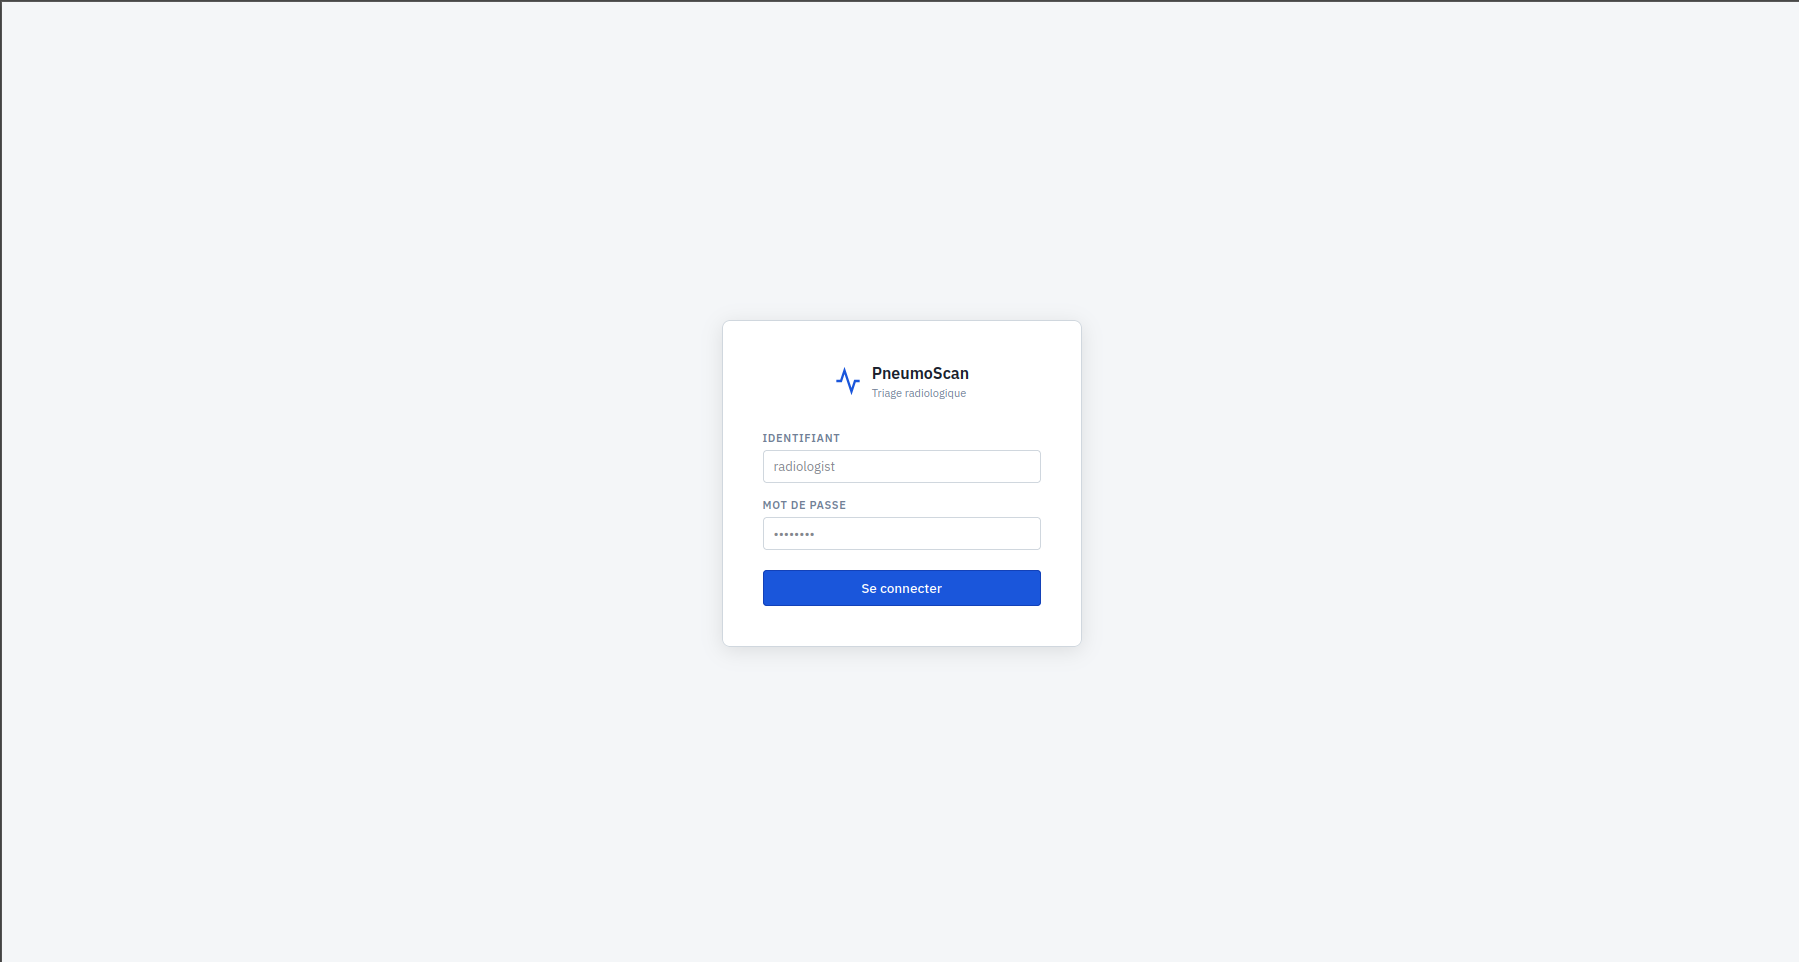
\includegraphics[width=0.92\textwidth]{assets/ui_login.png}
\caption{Écran de connexion (authentification JWT)}
\end{figure}

L'écran de connexion matérialise le besoin \textbf{BF-01} :
l'utilisateur saisit ses identifiants, le backend valide les credentials,
puis retourne un token \acrshort{jwt} signé qui servira à l'ensemble des appels protégés.

\begin{figure}[H]
\centering
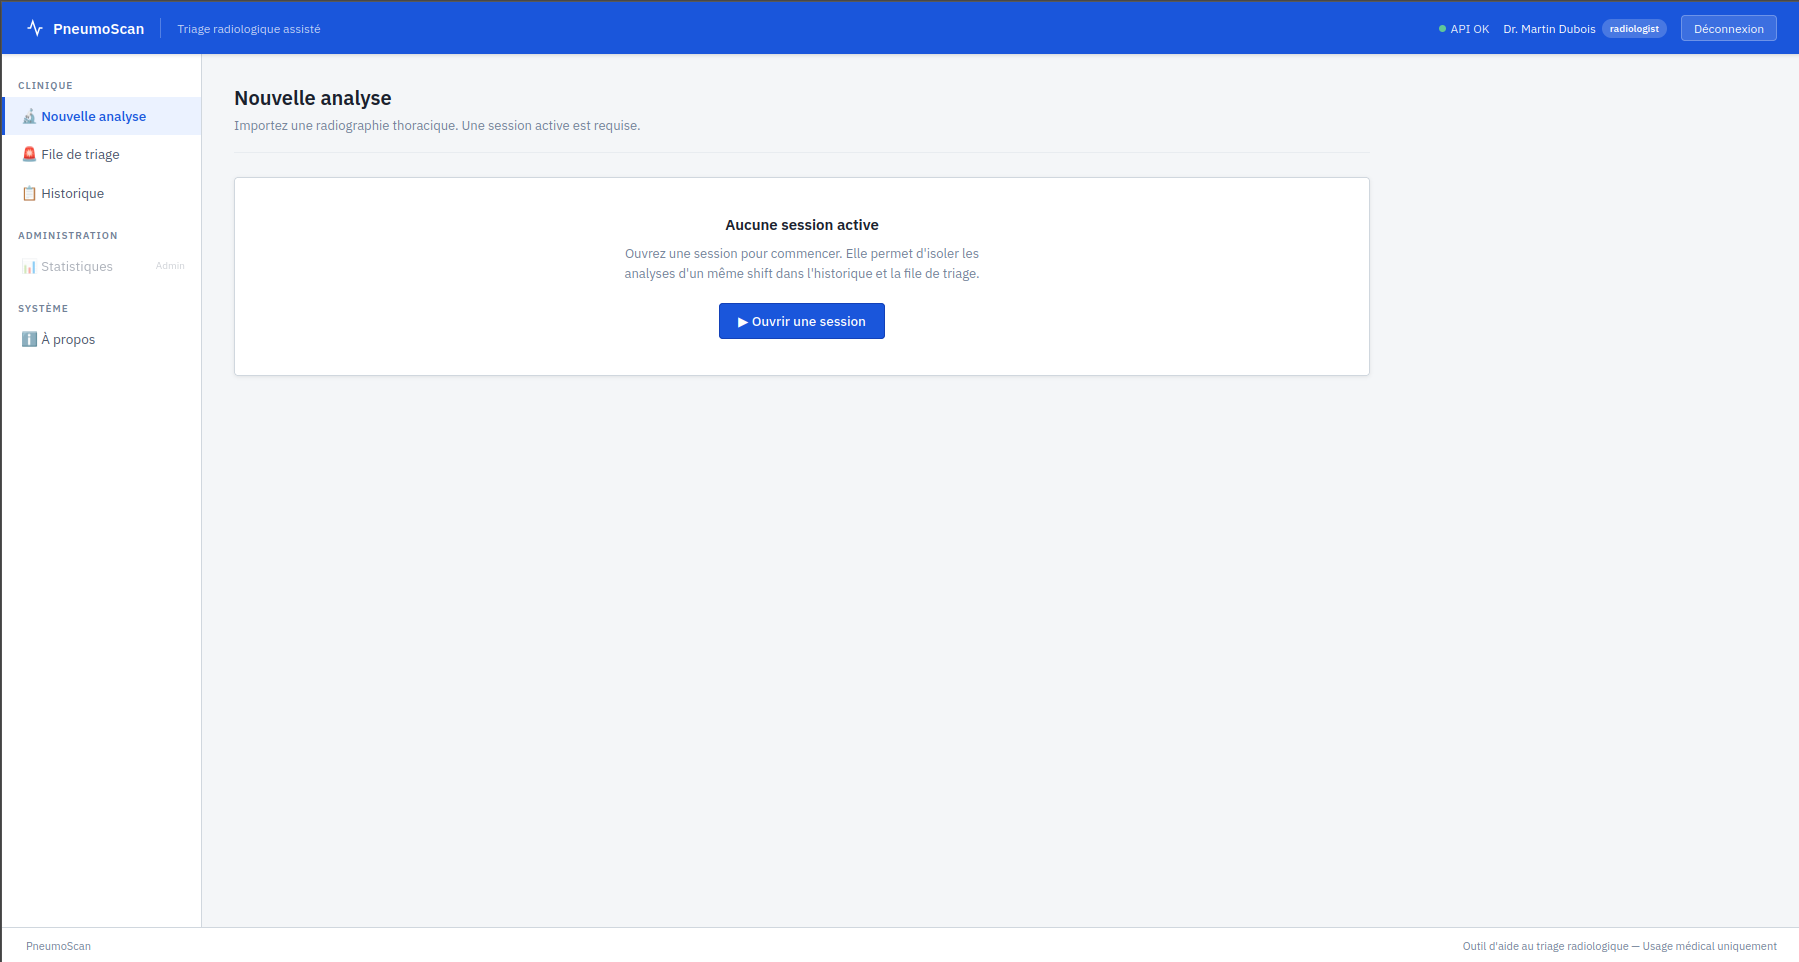
\includegraphics[width=0.92\textwidth]{assets/ui_new_analysis_no_session.png}
\caption{Nouvelle analyse sans session active}
\end{figure}

Cette vue montre la contrainte opérationnelle de traçabilité : sans session active,
l'analyse est bloquée. Cela garantit que chaque prédiction est rattachée à un shift
et à un opérateur, conformément aux besoins \textbf{BF-05} à \textbf{BF-08}.

\subsubsection{Analyse radiographique et explicabilité}

\begin{figure}[H]
\centering
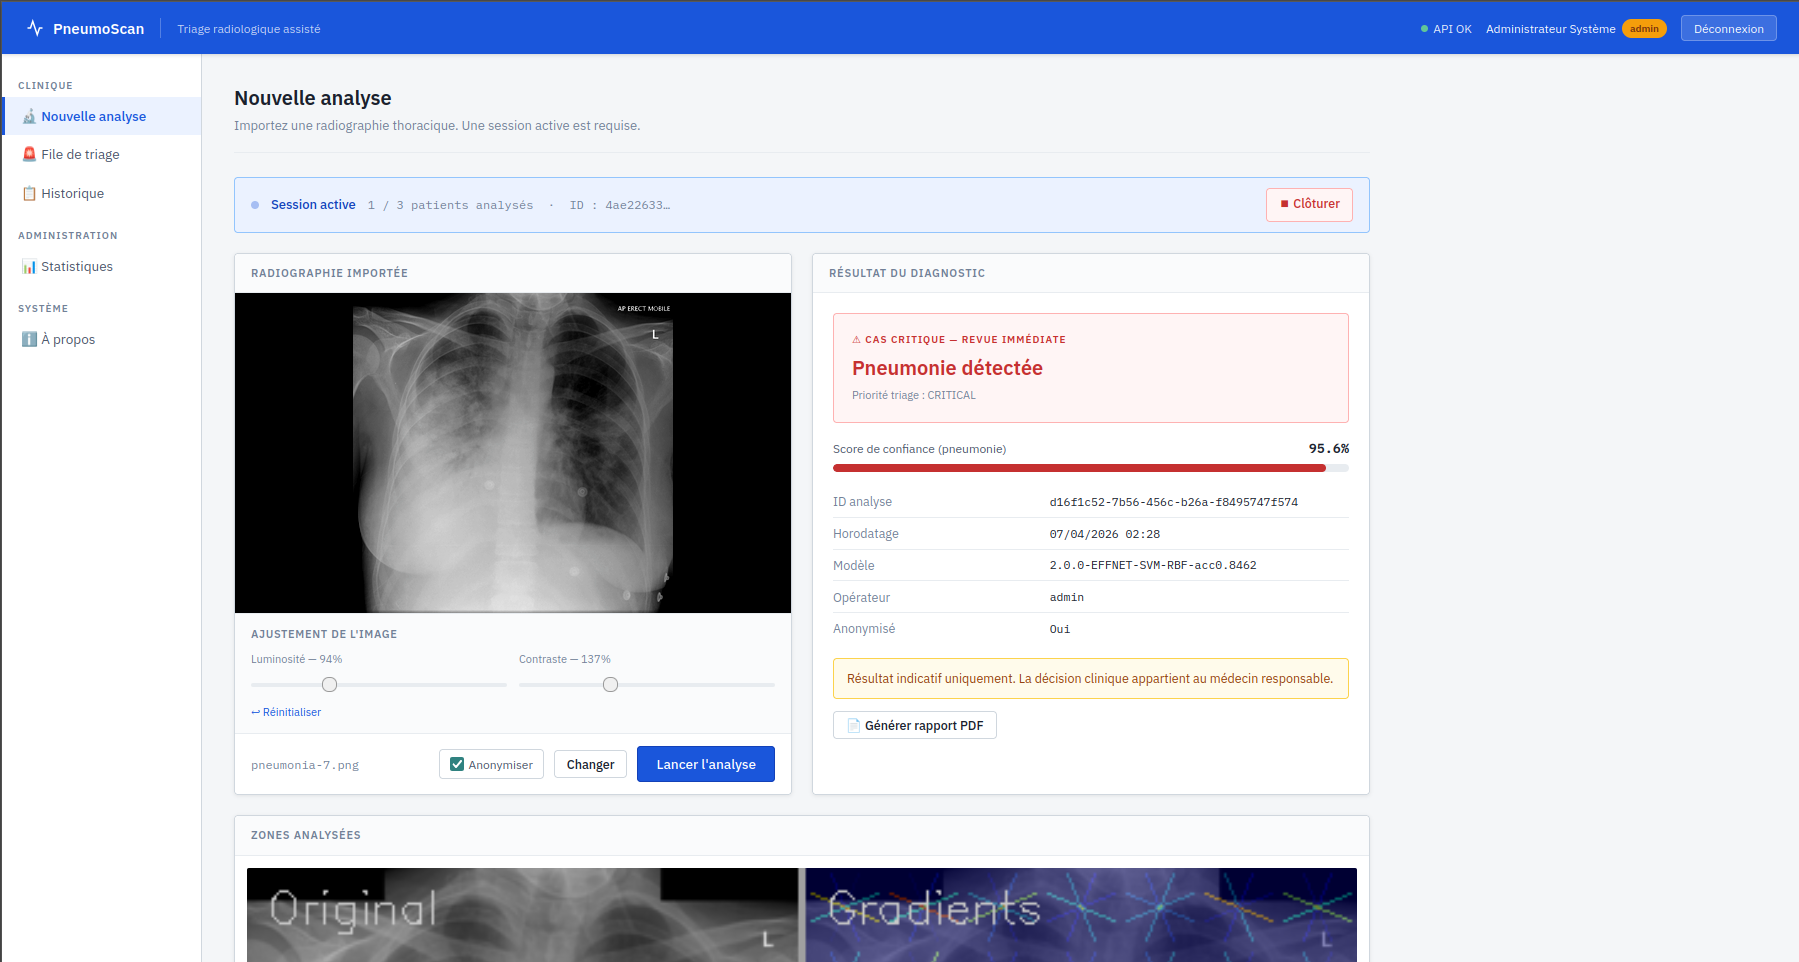
\includegraphics[width=0.92\textwidth]{assets/ui_analysis_result.png}
\caption{Écran d'analyse : image importée, résultat, score et triage}
\end{figure}

Cette interface regroupe le coeur métier : import de la radiographie,
anonymisation optionnelle, lancement du pipeline IA, affichage du label,
du score de confiance et du niveau de triage.
Elle couvre les besoins \textbf{BF-09} à \textbf{BF-12}.

\begin{figure}[H]
\centering
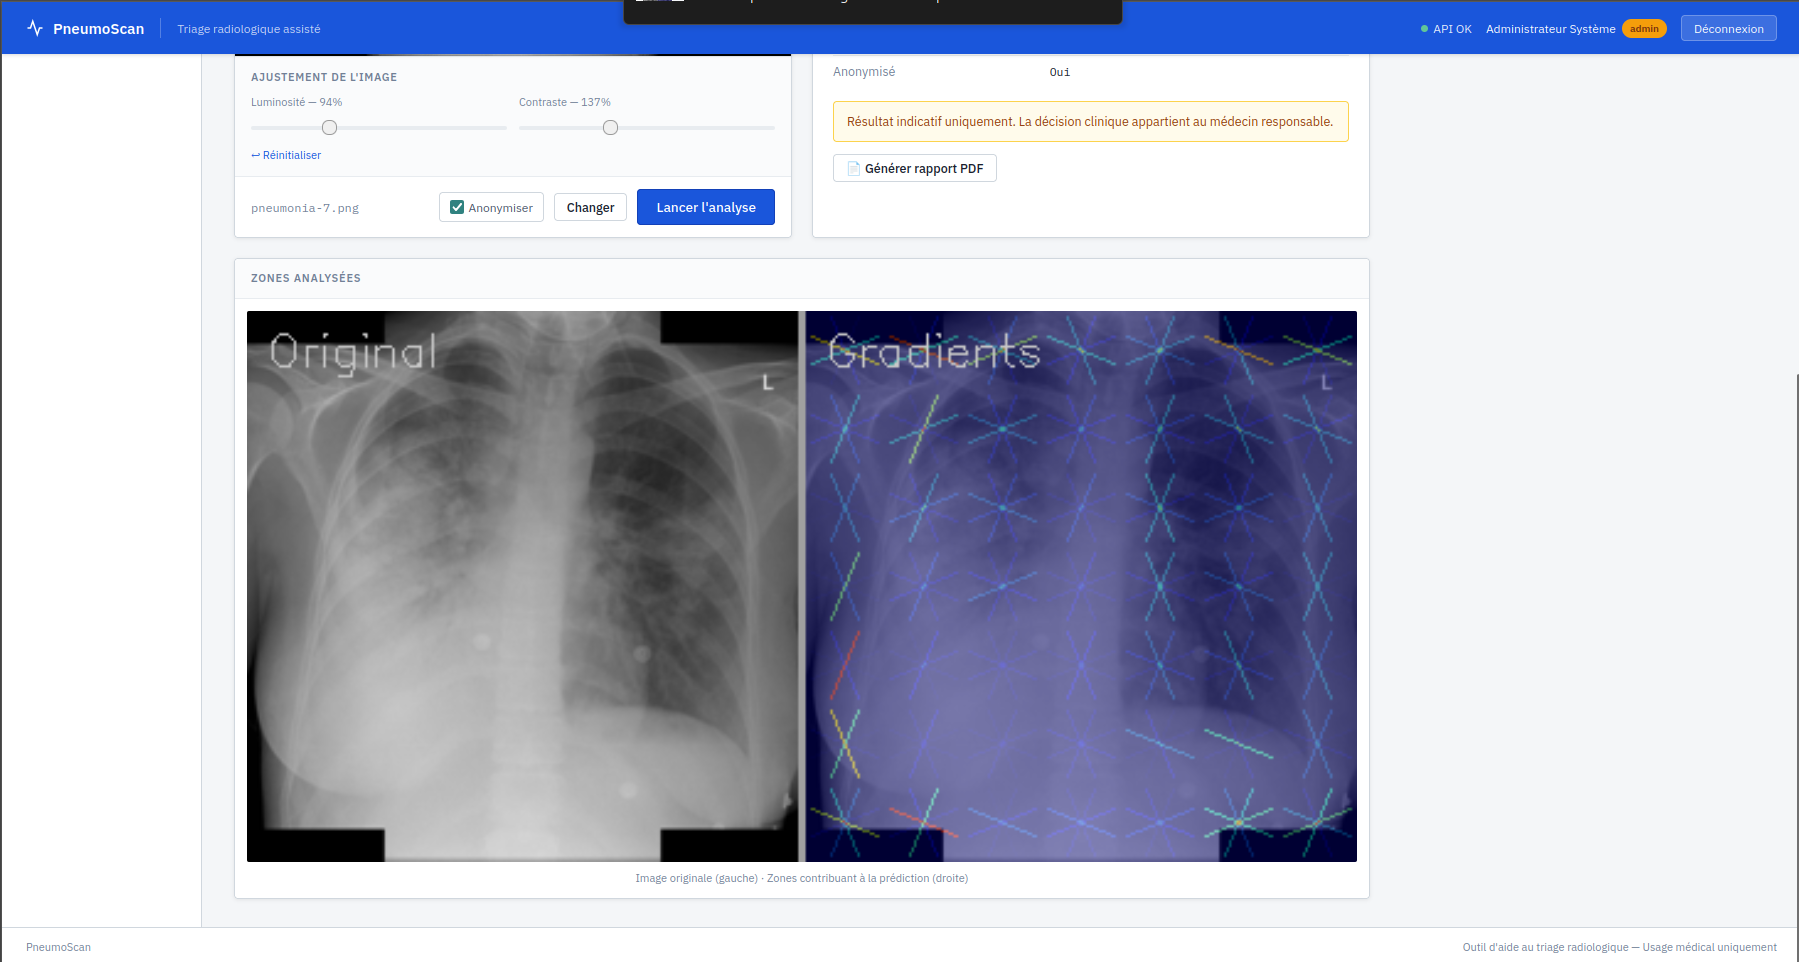
\includegraphics[width=0.92\textwidth]{assets/ui_analyzed_zones.png}
\caption{Zones analysées : comparaison image originale / gradients contributifs}
\end{figure}

La vue ``Zones analysées'' apporte une forme d'explicabilité visuelle :
les motifs de gradients les plus contributifs sont superposés à l'image,
ce qui facilite l'interprétation humaine et la discussion pédagogique du résultat.

\begin{figure}[H]
\centering
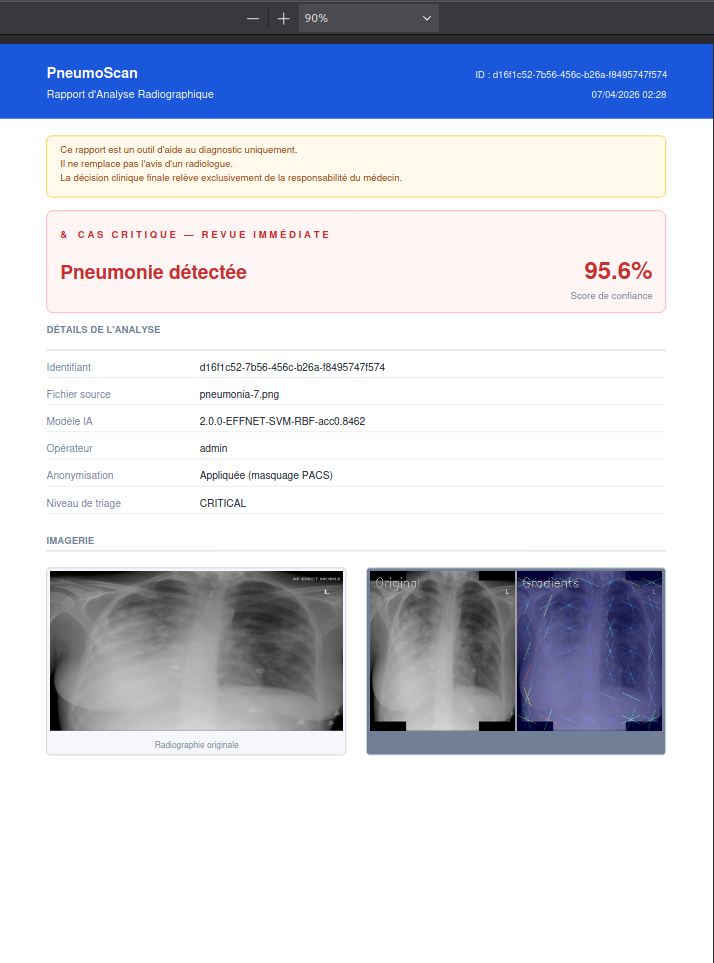
\includegraphics[width=0.7\textwidth]{assets/ui_pdf_report.png}
\caption{Rapport PDF généré automatiquement après analyse}
\end{figure}

Le rapport PDF formalise la sortie de l'analyse : identité technique,
récapitulatif du résultat, niveau de triage, images source et zones contributives.
Il constitue une trace exportable et consultable hors application.

\subsubsection{Pilotage clinique : file de triage, historique et supervision}

\begin{figure}[H]
\centering
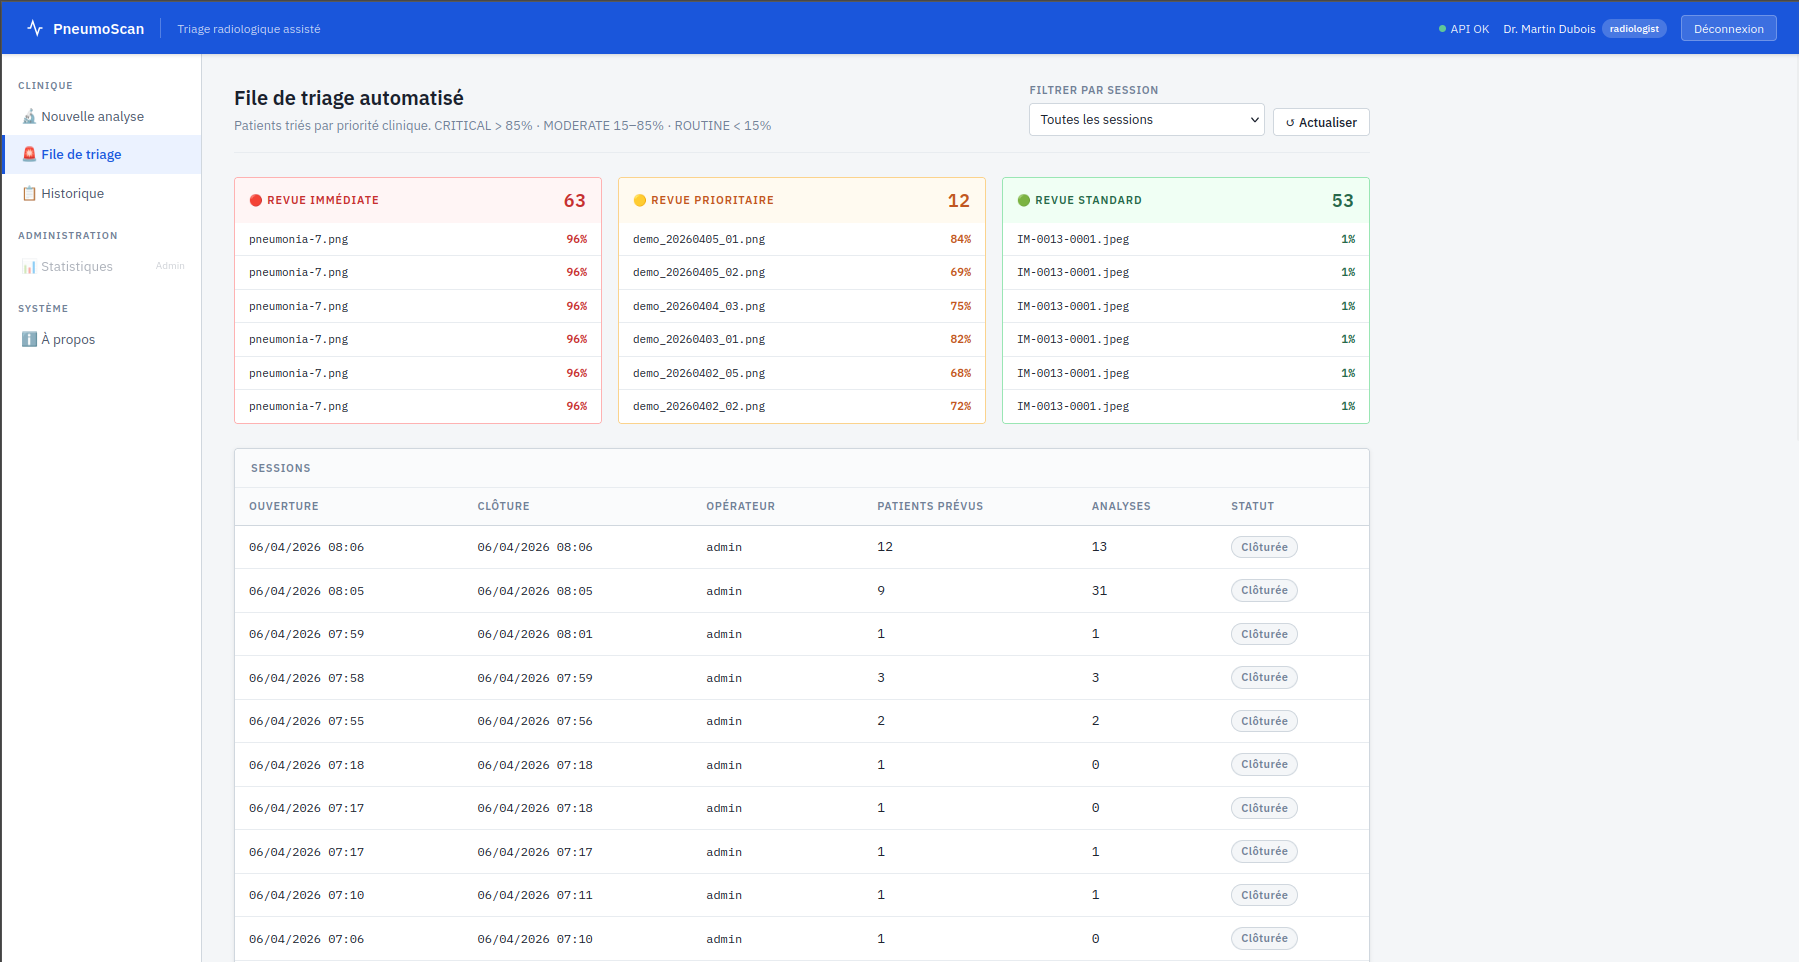
\includegraphics[width=0.92\textwidth]{assets/ui_triage_queue.png}
\caption{File de triage avec regroupement CRITICAL / MODERATE / ROUTINE}
\end{figure}

La file de triage met en oeuvre la priorisation clinique :
les cas critiques sont exposés en tête avec une mise en forme d'alerte,
les cas modérés sont orientés en revue prioritaire,
et les cas routiniers restent en revue standard.

\begin{figure}[H]
\centering
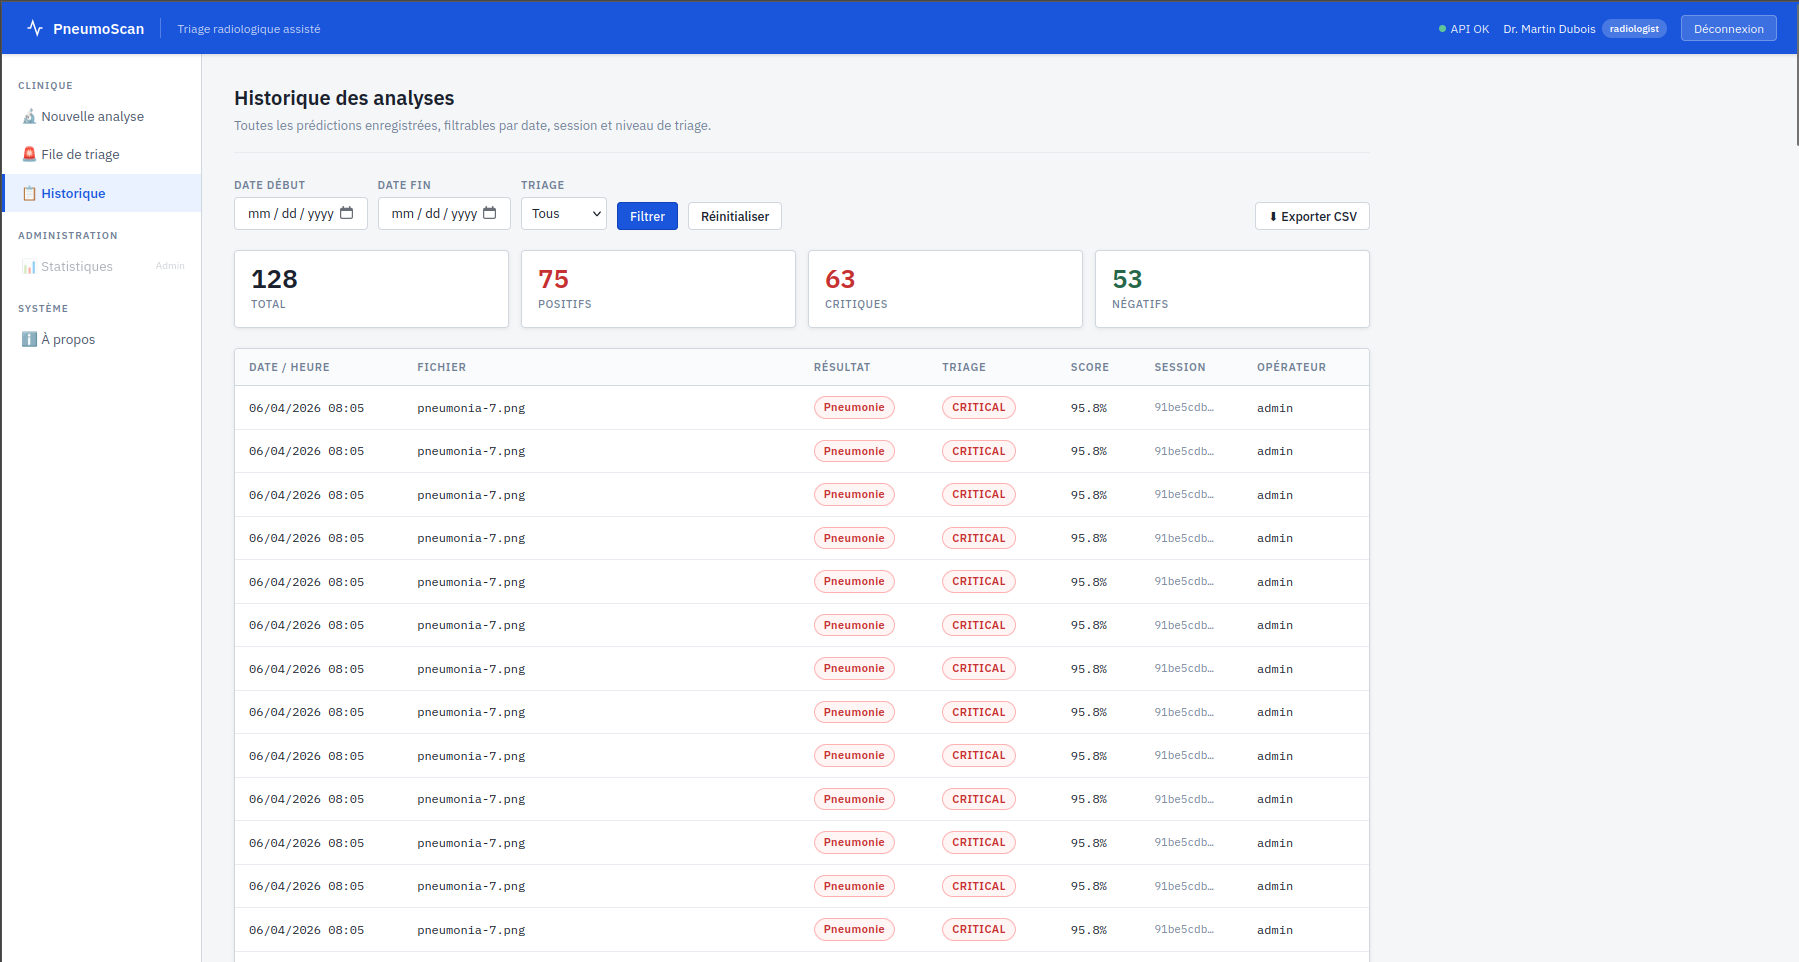
\includegraphics[width=0.92\textwidth]{assets/ui_history.png}
\caption{Historique filtrable des analyses et export CSV}
\end{figure}

L'historique assure la traçabilité temporelle complète :
filtrage par période et niveau de triage, consultation des scores,
et export CSV pour exploitation ultérieure.

\begin{figure}[H]
\centering
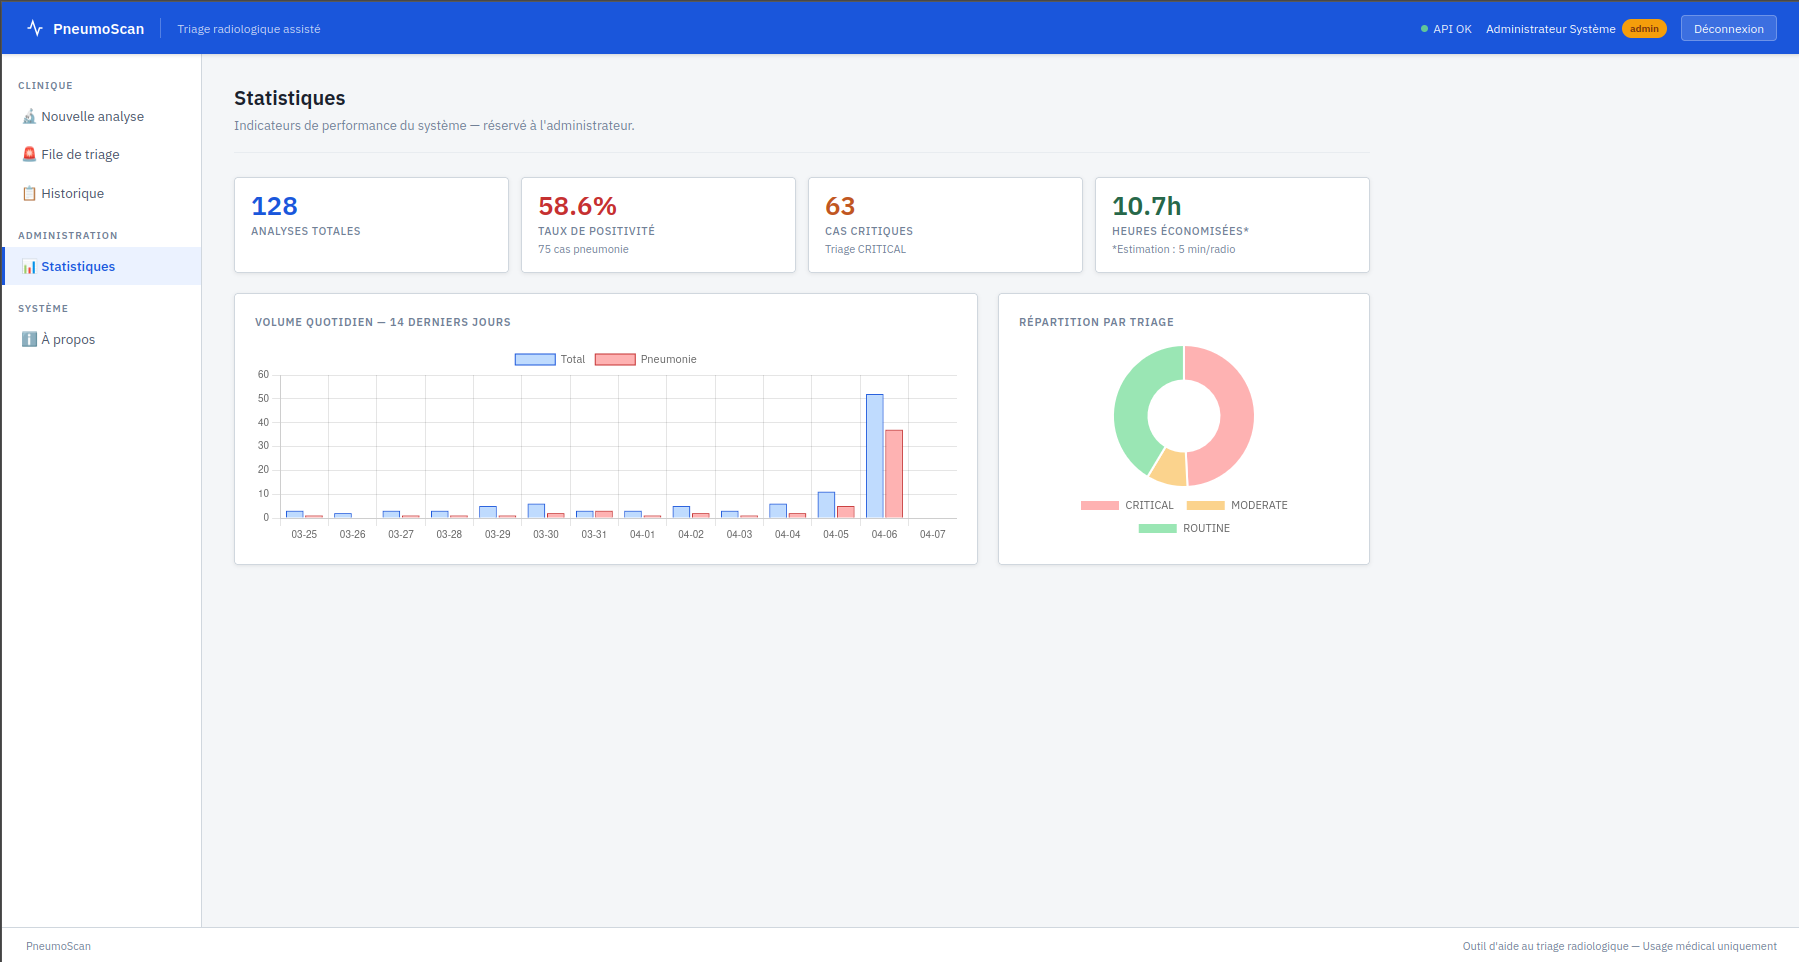
\includegraphics[width=0.92\textwidth]{assets/ui_admin_stats.png}
\caption{Tableau de bord administrateur (KPIs et graphiques BI)}
\end{figure}

Cette vue est réservée au rôle \texttt{admin}. Elle agrège les indicateurs
de performance du service : volume, positivité, proportion de cas critiques,
et estimation des heures économisées.

\begin{figure}[H]
\centering
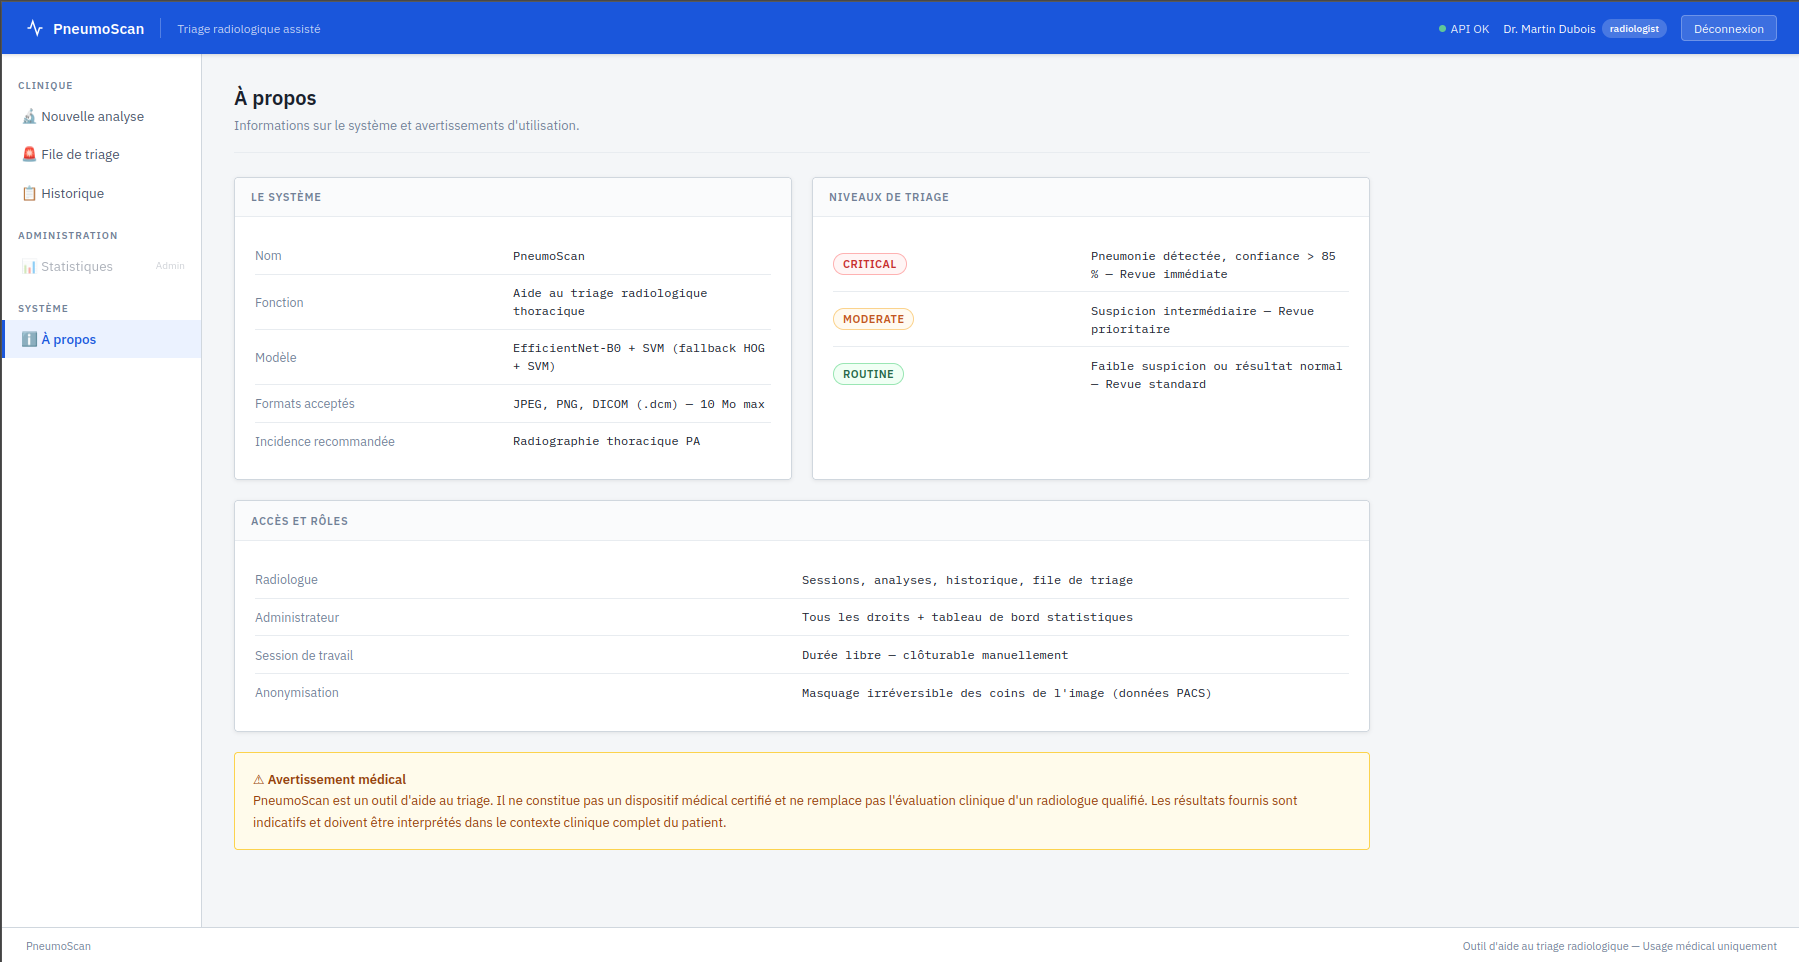
\includegraphics[width=0.92\textwidth]{assets/ui_about.png}
\caption{Page ``À propos'' : périmètre d'usage, niveaux de triage et avertissement médical}
\end{figure}

La page ``À propos'' rappelle le périmètre du prototype,
les formats supportés, les rôles applicatifs et l'avertissement médical.
Elle joue un rôle essentiel de transparence et de bon usage.

\section{Analyse Non Fonctionnelle}

\begin{table}[H]
\centering
\caption{Besoins non fonctionnels}
\begin{tabularx}{\textwidth}{L{1.5cm} L{3.5cm} X}
\toprule
\textbf{ID} & \textbf{Catégorie} & \textbf{Exigence} \\
\midrule
BNF-01 & Performance &
  Temps de réponse de \texttt{/predict} inférieur à 3 secondes pour une image standard. \\
BNF-02 & Sécurité &
  Tokens JWT signés HS256 via variable d'environnement. Mots de passe hachés bcrypt. \\
BNF-03 & Disponibilité &
  Endpoint \texttt{GET /health} + healthcheck Docker (intervalle 30s). \\
BNF-04 & Maintenabilité &
  Docstrings exhaustifs sur tous les modules. 32 tests unitaires pytest (5 classes). \\
BNF-05 & Portabilité &
  Déploiement Docker Compose reproductible en une commande. \\
BNF-06 & Conformité RGPD &
  Anonymisation par masquage noir irréversible. Aucune donnée nominative stockée. \\
BNF-07 & Accessibilité &
  Interface responsive (mobile/desktop). Contraste WCAG AA respecté. \\
\bottomrule
\end{tabularx}
\end{table}

\section{Acteurs et Rôles}

\begin{table}[H]
\centering
\caption{Acteurs du système et leurs responsabilités}
\begin{tabularx}{\textwidth}{L{3cm} L{2.5cm} X}
\toprule
\textbf{Acteur} & \textbf{Rôle JWT} & \textbf{Responsabilités} \\
\midrule
Radiologue & \texttt{radiologist} &
  Crée les sessions, soumet les radiographies, consulte la file de triage et l'historique \\
Administrateur & \texttt{admin} &
  Tous les droits du radiologue + accès exclusif au tableau de bord BI \\
Système IA & (interne) &
  Exécute le pipeline de validation OOD, extraction de features et classification SVM \\
\bottomrule
\end{tabularx}
\end{table}

\subsection{Rôle de supervision (administrateur)}

Dans le contexte de PneumoScan, l'\textbf{administrateur} joue le rôle
de supervision : il accède aux statistiques globales du service de radiologie,
suit les indicateurs de performance et peut consulter l'ensemble des sessions
de tous les opérateurs.

\subsection{Rôle opérationnel (radiologue)}

Le \textbf{radiologue} est l'utilisateur principal du système. Il réalise
les analyses, gère ses sessions de travail et consulte la file de triage
pour optimiser son workflow de lecture.

\subsection{Administrateur}

L'administrateur dispose de l'ensemble des droits du radiologue,
augmentés de l'accès au tableau de bord BI. Il est identifiable par le token
JWT portant le rôle \texttt{admin}.

\section{Acteurs et Cas d'Utilisation}

\subsection{Diagramme de cas d'utilisation}

Le diagramme ci-dessous représente les cas d'utilisation principaux du système :

\begin{figure}[H]
\centering
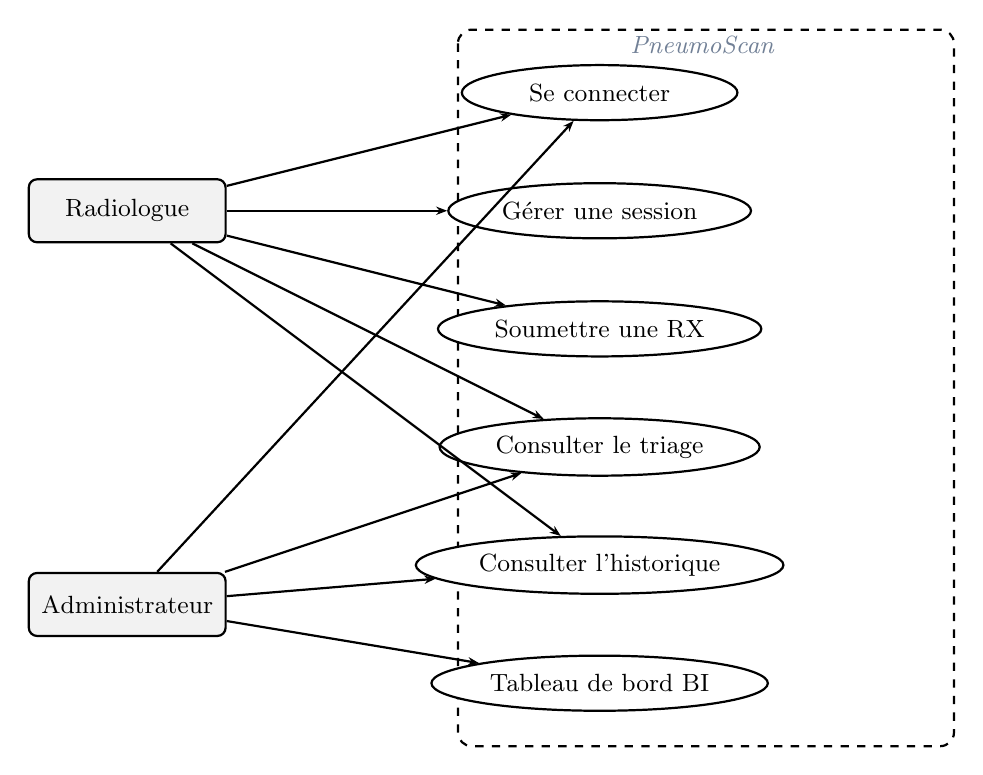
\begin{tikzpicture}[
  actor/.style={rectangle, draw, thick, minimum width=2.5cm, minimum height=0.8cm,
                rounded corners=3pt, fill=gray!10},
  usecase/.style={ellipse, draw, thick, minimum width=3.5cm, minimum height=0.7cm,
                  fill=white, font=\small},
  arrow/.style={-{Stealth[length=4pt]}, thick},
  include/.style={-{Stealth[length=4pt]}, dashed, thick},
  every node/.style={font=\small},
]
  % Acteurs
  \node[actor] (radio) at (-4, 0) {Radiologue};
  \node[actor] (admin) at (-4, -5) {Administrateur};

  % Cas d'utilisation
  \node[usecase] (login) at (2, 1.5) {Se connecter};
  \node[usecase] (session) at (2, 0) {Gérer une session};
  \node[usecase] (analyse) at (2, -1.5) {Soumettre une RX};
  \node[usecase] (triage) at (2, -3) {Consulter le triage};
  \node[usecase] (history) at (2, -4.5) {Consulter l'historique};
  \node[usecase] (dashboard) at (2, -6) {Tableau de bord BI};

  % Connexions radiologue
  \draw[arrow] (radio) -- (login);
  \draw[arrow] (radio) -- (session);
  \draw[arrow] (radio) -- (analyse);
  \draw[arrow] (radio) -- (triage);
  \draw[arrow] (radio) -- (history);

  % Connexions administrateur
  \draw[arrow] (admin) -- (login);
  \draw[arrow] (admin) -- (dashboard);
  \draw[arrow] (admin) -- (triage);
  \draw[arrow] (admin) -- (history);

  % Frontière système
  \begin{scope}[on background layer]
    \draw[dashed, thick, rounded corners=5pt]
      (0.2, 2.3) rectangle (6.5, -6.8);
    \node[font=\small\itshape, text=muted] at (3.3, 2.1) {PneumoScan};
  \end{scope}
\end{tikzpicture}
\caption{Diagramme de cas d'utilisation global}
\end{figure}
\newpage
\section{Description des Cas d'Utilisation}

\subsection{Pour les Utilisateurs}

\subsubsection{Se connecter / Se déconnecter}

\begin{table}[H]
\centering
\caption{CU-01 --- Se connecter}
\begin{tabularx}{\textwidth}{L{3.5cm} X}
\toprule
\textbf{Acteur principal} & Radiologue / Administrateur \\
\textbf{Précondition} & L'utilisateur possède un compte valide \\
\textbf{Scénario nominal} & 1. L'utilisateur saisit son identifiant et mot de passe \\
 & 2. Le backend valide les identifiants et génère un token JWT \\
 & 3. Le frontend stocke le token dans le \texttt{sessionStorage} \\
 & 4. L'interface principale est affichée \\
\textbf{Scénario alternatif} & Identifiants incorrects → message d'erreur inline \\
\textbf{Postcondition} & Token JWT valide, sessions fantômes clôturées \\
\bottomrule
\end{tabularx}
\end{table}

\subsection{Publication, Recherche et Interaction}

\subsubsection{Soumettre une radiographie pour analyse}

\begin{table}[H]
\centering
\caption{CU-02 --- Soumettre une radiographie}
\begin{tabularx}{\textwidth}{L{3.5cm} X}
\toprule
\textbf{Acteur principal} & Radiologue \\
\textbf{Précondition} & Session active ouverte, token JWT valide \\
\textbf{Scénario nominal} & 1. Le radiologue dépose un fichier JPEG/PNG/DICOM (.dcm) \\
 & 2. Le frontend prévisualise le cliché \\
 & 3. Le radiologue clique sur ``Lancer l'analyse'' \\
 & 4. L'API valide le format et applique la garde OOD \\
 & 5. Le pipeline EfficientNet-B0+SVM est exécuté (fallback HOG+SVM si artefact absent) \\
 & 6. Le résultat (label, score, niveau de triage) est retourné \\
 & 7. La carte d'attention HOG est générée et affichée \\
 & 8. La prédiction est persistée en base de données \\
\textbf{Exception} & Image non radiographique → HTTP 400 + message d'erreur inline \\
\textbf{Postcondition} & Prédiction stockée, file de triage mise à jour \\
\bottomrule
\end{tabularx}
\end{table}

\subsection{Paiement et Évaluation}

Dans PneumoScan, cette dimension correspond à l'\textbf{évaluation des performances}
du système via le tableau de bord BI et la génération de rapports PDF,
qui constituent la trace formelle de chaque analyse.

\section{Diagramme de cas d'utilisation}

Voir figure 2.1 en section 2.5.

\section{Conclusion du Chapitre}

Ce chapitre a défini les acteurs, les besoins fonctionnels et non fonctionnels,
et les principaux cas d'utilisation du système. Le chapitre suivant aborde
la conception et la réalisation technique de PneumoScan.

% ============================================================
% CHAPITRE 3 --- CONCEPTION ET REALISATION
% ============================================================
\chapter{Conception et Réalisation}

\section{Introduction}

Ce chapitre présente la conception détaillée et la réalisation de PneumoScan.
Il suit la structure UML définie en phase d'élaboration et documente les choix
d'implémentation de chaque composant.

\section{Architecture Logicielle Refactorisée (Clean Code \& SOLID)}

Afin d'améliorer la maintenabilité, la robustesse et la lisibilité du projet
en vue d'une soutenance technique, une refactorisation architecturale a été
réalisée selon une séparation explicite des responsabilités.

\begin{table}[H]
\centering
\caption{Organisation modulaire du backend après refactorisation}
\begin{tabularx}{\textwidth}{L{3.2cm} L{3.8cm} X}
\toprule
\textbf{Couche} & \textbf{Fichiers} & \textbf{Responsabilité principale} \\
\midrule
Contrôleurs HTTP & \texttt{main.py} & Déclaration des routes FastAPI, validation des entrées HTTP, mapping des exceptions vers les codes d'erreur API \\
Services applicatifs & \texttt{services.py} & Orchestration des cas d'usage (analyse, sessions, historique, dashboard) sans dépendance au transport HTTP \\
Configuration & \texttt{settings.py} & Centralisation des paramètres d'exécution (version, répertoire heatmaps, CORS) \\
Sécurité & \texttt{auth.py} & Authentification JWT, RBAC, dépendances FastAPI de contrôle d'accès \\
Données & \texttt{database.py} & Persistance SQLite, règles de triage, agrégations BI, gestion des sessions \\
ML \& image & \texttt{predictor.py} & Validation OOD, prétraitement, extraction HOG, inférence SVM, génération heatmap, anonymisation \\
Validation & \texttt{utils.py} & Validation uniforme des métadonnées d'upload et des contraintes de taille \\
\bottomrule
\end{tabularx}
\end{table}

\begin{infobox}[Justification SOLID]
\begin{itemize}
  \item \textbf{S (Single Responsibility):} chaque module a un rôle unique (ex. \texttt{services.py} n'implémente pas de logique SQL directe).
  \item \textbf{O (Open/Closed):} l'ajout d'une nouvelle stratégie d'analyse peut être fait dans la couche service sans modifier les routes existantes.
  \item \textbf{L (Liskov):} les fonctions de service exposent des contrats stables consommés par les contrôleurs.
  \item \textbf{I (Interface Segregation):} les dépendances FastAPI utilisent des interfaces de rôle dédiées (\texttt{require\_radiologist}, \texttt{require\_admin}).
  \item \textbf{D (Dependency Inversion):} \texttt{main.py} dépend d'abstractions de service (cas d'usage), et non de détails de persistance ou de traitement image.
\end{itemize}
\end{infobox}

\section{Diagrammes des Séquences}

\subsection{Connexion}

\begin{figure}[H]
\centering
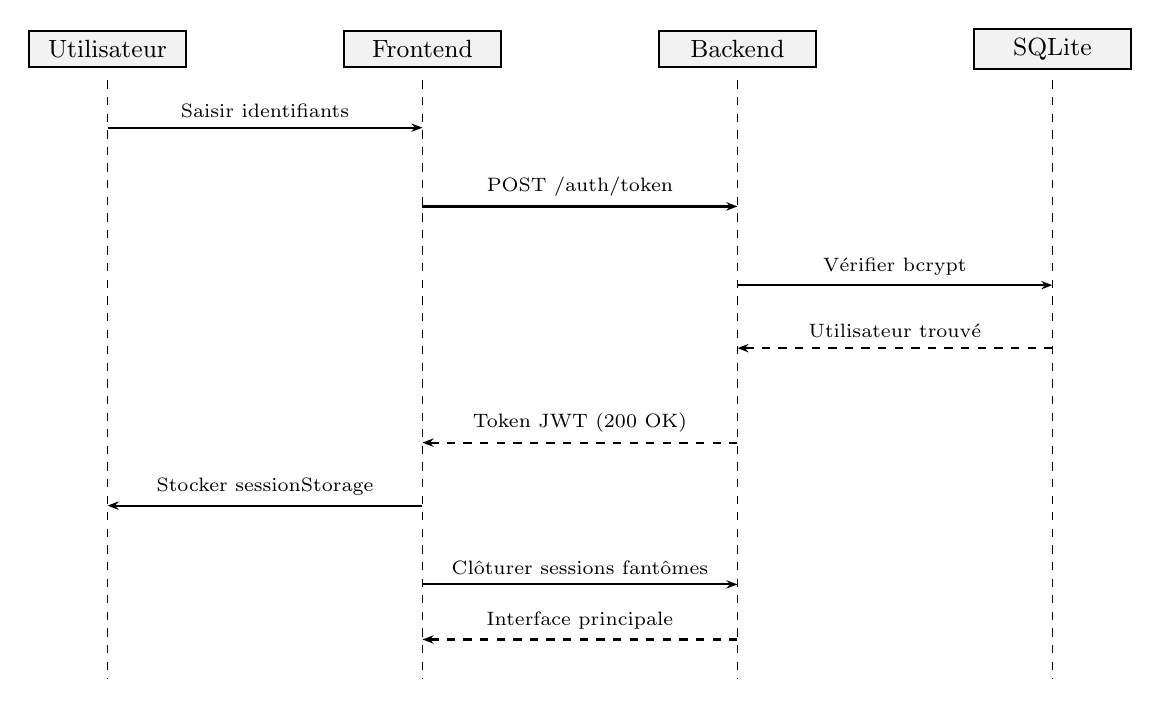
\begin{tikzpicture}[
  every node/.style={font=\small},
  lifeline/.style={thick},
  msg/.style={-{Stealth[length=4pt]}, thick},
  ret/.style={-{Stealth[length=4pt]}, thick, dashed},
]
  % En-têtes acteurs
  \node[rectangle, draw, thick, fill=gray!10, minimum width=2cm] (U) at (0,0) {Utilisateur};
  \node[rectangle, draw, thick, fill=gray!10, minimum width=2cm] (FE) at (4,0) {Frontend};
  \node[rectangle, draw, thick, fill=gray!10, minimum width=2cm] (BE) at (8,0) {Backend};
  \node[rectangle, draw, thick, fill=gray!10, minimum width=2cm] (DB) at (12,0) {SQLite};

  % Lignes de vie
  \draw[dashed] (0,-0.4) -- (0,-8);
  \draw[dashed] (4,-0.4) -- (4,-8);
  \draw[dashed] (8,-0.4) -- (8,-8);
  \draw[dashed] (12,-0.4) -- (12,-8);

  % Messages
  \draw[msg] (0,-1) -- node[above,font=\scriptsize]{Saisir identifiants} (4,-1);
  \draw[msg] (4,-2) -- node[above,font=\scriptsize]{POST /auth/token} (8,-2);
  \draw[msg] (8,-3) -- node[above,font=\scriptsize]{Vérifier bcrypt} (12,-3);
  \draw[ret] (12,-3.8) -- node[above,font=\scriptsize]{Utilisateur trouvé} (8,-3.8);
  \draw[ret] (8,-5) -- node[above,font=\scriptsize]{Token JWT (200 OK)} (4,-5);
  \draw[msg] (4,-5.8) -- node[above,font=\scriptsize]{Stocker sessionStorage} (0,-5.8);
  \draw[msg] (4,-6.8) -- node[above,font=\scriptsize]{Clôturer sessions fantômes} (8,-6.8);
  \draw[ret] (8,-7.5) -- node[above,font=\scriptsize]{Interface principale} (4,-7.5);
\end{tikzpicture}
\caption{Diagramme de séquence --- Connexion}
\end{figure}

\subsection{Inscription}

L'inscription n'est pas disponible en mode libre dans ce prototype.
Les comptes sont pré-configurés en mémoire (phase prototype).
En production, un endpoint \texttt{POST /auth/register} permettrait
la création de comptes avec validation par un administrateur.

\subsection{Soumettre une radiographie}

Dans le contexte de PneumoScan : \textbf{soumettre une radiographie pour analyse}.
Voir le diagramme de séquence détaillé ci-dessous.

\begin{figure}[H]
\centering
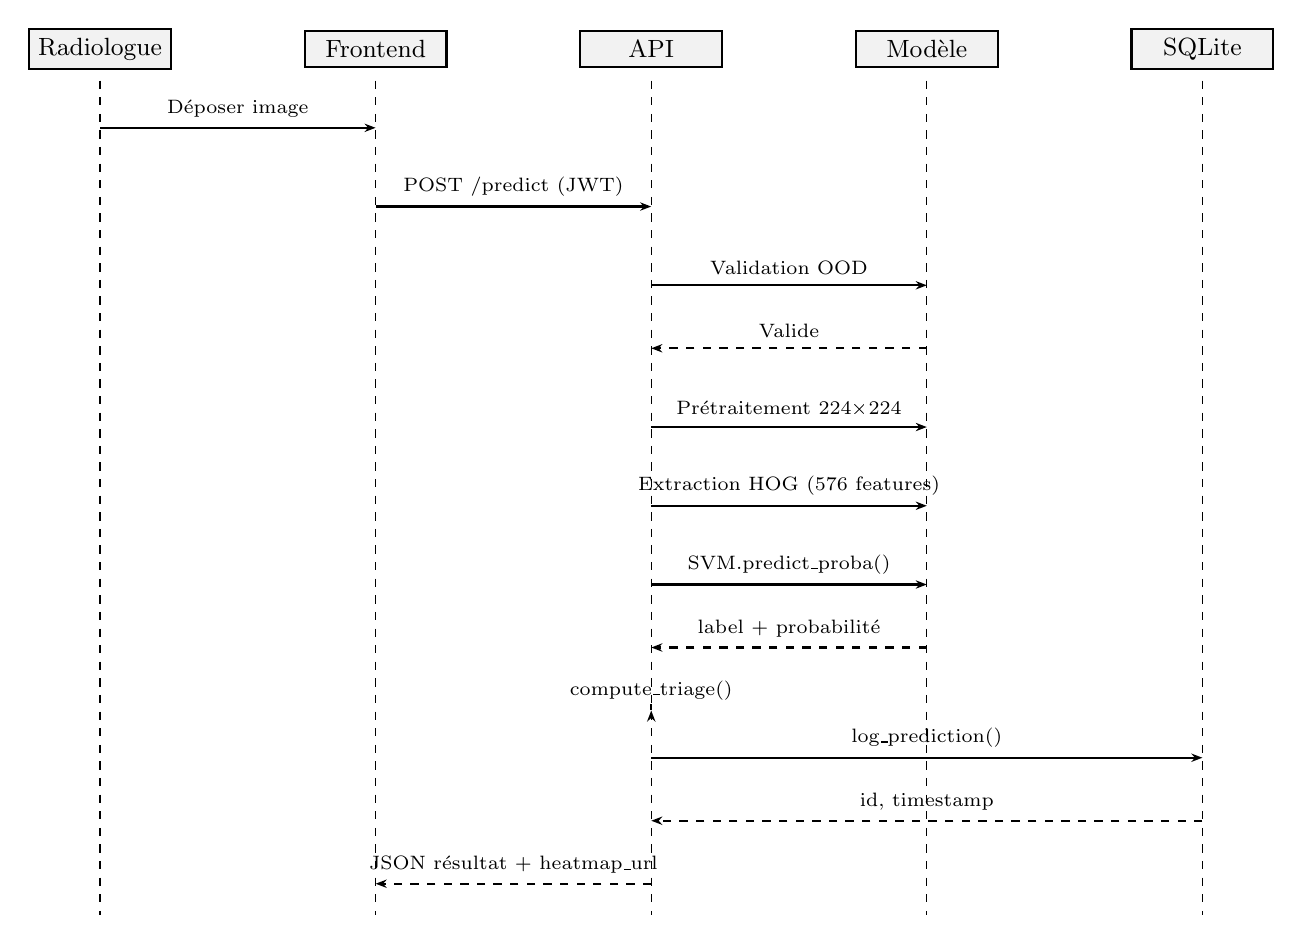
\begin{tikzpicture}[
  every node/.style={font=\small},
  msg/.style={-{Stealth[length=4pt]}, thick},
  ret/.style={-{Stealth[length=4pt]}, thick, dashed},
  guard/.style={rectangle, draw, fill=orange!10, font=\scriptsize},
]
  \node[rectangle,draw,thick,fill=gray!10,minimum width=1.8cm] (R) at (0,0) {Radiologue};
  \node[rectangle,draw,thick,fill=gray!10,minimum width=1.8cm] (FE) at (3.5,0) {Frontend};
  \node[rectangle,draw,thick,fill=gray!10,minimum width=1.8cm] (BE) at (7,0) {API};
  \node[rectangle,draw,thick,fill=gray!10,minimum width=1.8cm] (ML) at (10.5,0) {Modèle};
  \node[rectangle,draw,thick,fill=gray!10,minimum width=1.8cm] (DB) at (14,0) {SQLite};

  \draw[dashed] (0,-0.4) -- (0,-11);
  \draw[dashed] (3.5,-0.4) -- (3.5,-11);
  \draw[dashed] (7,-0.4) -- (7,-11);
  \draw[dashed] (10.5,-0.4) -- (10.5,-11);
  \draw[dashed] (14,-0.4) -- (14,-11);

  \draw[msg] (0,-1) -- node[above,font=\scriptsize]{Déposer image} (3.5,-1);
  \draw[msg] (3.5,-2) -- node[above,font=\scriptsize]{POST /predict (JWT)} (7,-2);
  \draw[msg] (7,-3) -- node[above,font=\scriptsize]{Validation OOD} (10.5,-3);
  \draw[ret] (10.5,-3.8) -- node[above,font=\scriptsize]{Valide} (7,-3.8);
  \draw[msg] (7,-4.8) -- node[above,font=\scriptsize]{Prétraitement 224×224} (10.5,-4.8);
  \draw[msg] (7,-5.8) -- node[above,font=\scriptsize]{Extraction HOG (576 features)} (10.5,-5.8);
  \draw[msg] (7,-6.8) -- node[above,font=\scriptsize]{SVM.predict\_proba()} (10.5,-6.8);
  \draw[ret] (10.5,-7.6) -- node[above,font=\scriptsize]{label + probabilité} (7,-7.6);
  \draw[msg] (7,-8.4) -- node[above,font=\scriptsize]{compute\_triage()} (7,-8.4);
  \draw[msg] (7,-9) -- node[above,font=\scriptsize]{log\_prediction()} (14,-9);
  \draw[ret] (14,-9.8) -- node[above,font=\scriptsize]{id, timestamp} (7,-9.8);
  \draw[ret] (7,-10.6) -- node[above,font=\scriptsize]{JSON résultat + heatmap\_url} (3.5,-10.6);
\end{tikzpicture}
\caption{Diagramme de séquence --- Analyse radiographique}
\end{figure}

\subsection{Consulter mes activités}

\begin{figure}[H]
\centering
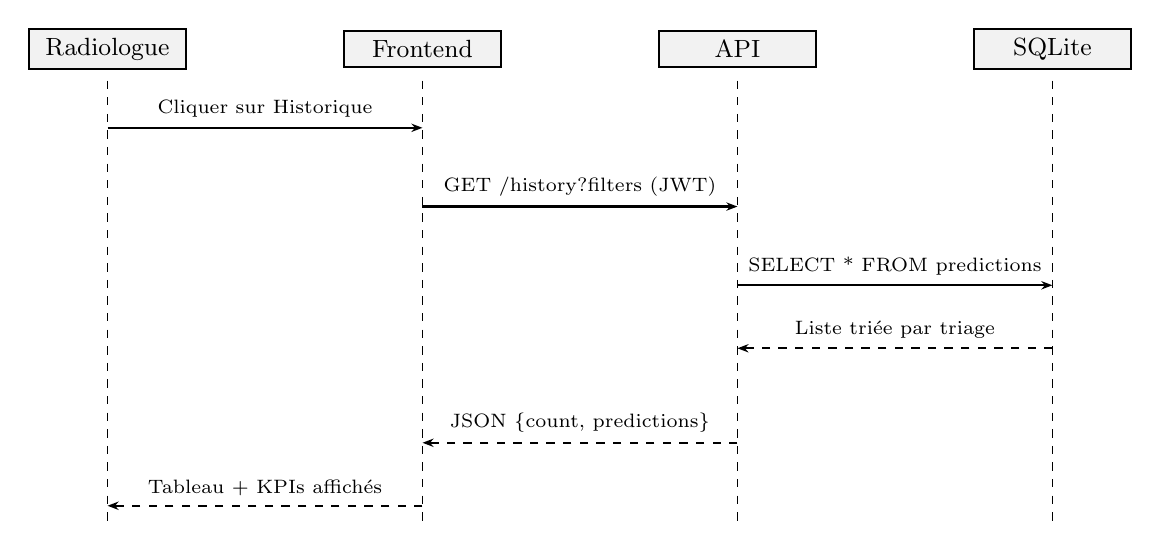
\begin{tikzpicture}[
  every node/.style={font=\small},
  msg/.style={-{Stealth[length=4pt]}, thick},
  ret/.style={-{Stealth[length=4pt]}, thick, dashed},
]
  \node[rectangle,draw,thick,fill=gray!10,minimum width=2cm] (R) at (0,0) {Radiologue};
  \node[rectangle,draw,thick,fill=gray!10,minimum width=2cm] (FE) at (4,0) {Frontend};
  \node[rectangle,draw,thick,fill=gray!10,minimum width=2cm] (BE) at (8,0) {API};
  \node[rectangle,draw,thick,fill=gray!10,minimum width=2cm] (DB) at (12,0) {SQLite};

  \draw[dashed] (0,-0.4) -- (0,-6);
  \draw[dashed] (4,-0.4) -- (4,-6);
  \draw[dashed] (8,-0.4) -- (8,-6);
  \draw[dashed] (12,-0.4) -- (12,-6);

  \draw[msg] (0,-1) -- node[above,font=\scriptsize]{Cliquer sur Historique} (4,-1);
  \draw[msg] (4,-2) -- node[above,font=\scriptsize]{GET /history?filters (JWT)} (8,-2);
  \draw[msg] (8,-3) -- node[above,font=\scriptsize]{SELECT * FROM predictions} (12,-3);
  \draw[ret] (12,-3.8) -- node[above,font=\scriptsize]{Liste triée par triage} (8,-3.8);
  \draw[ret] (8,-5) -- node[above,font=\scriptsize]{JSON \{count, predictions\}} (4,-5);
  \draw[ret] (4,-5.8) -- node[above,font=\scriptsize]{Tableau + KPIs affichés} (0,-5.8);
\end{tikzpicture}
\caption{Diagramme de séquence --- Consultation de l'historique}
\end{figure}

\subsection{Ouvrir une session de travail}

Dans PneumoScan : \textbf{ouvrir une session de travail}.

\begin{figure}[H]
\centering
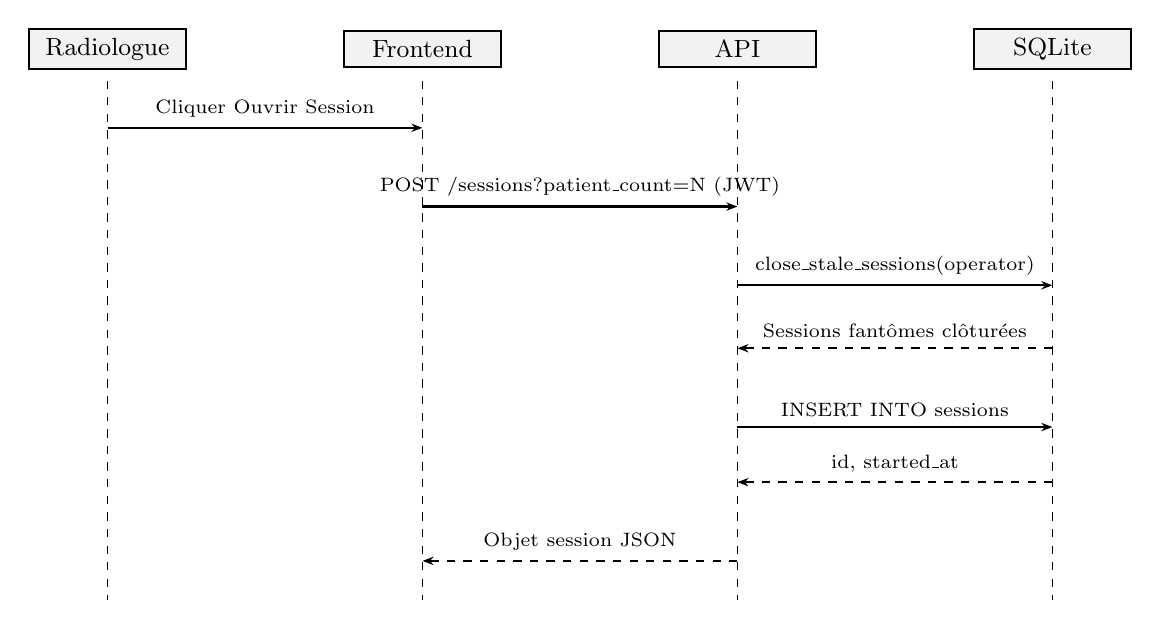
\begin{tikzpicture}[
  every node/.style={font=\small},
  msg/.style={-{Stealth[length=4pt]}, thick},
  ret/.style={-{Stealth[length=4pt]}, thick, dashed},
]
  \node[rectangle,draw,thick,fill=gray!10,minimum width=2cm] (R) at (0,0) {Radiologue};
  \node[rectangle,draw,thick,fill=gray!10,minimum width=2cm] (FE) at (4,0) {Frontend};
  \node[rectangle,draw,thick,fill=gray!10,minimum width=2cm] (BE) at (8,0) {API};
  \node[rectangle,draw,thick,fill=gray!10,minimum width=2cm] (DB) at (12,0) {SQLite};

  \draw[dashed] (0,-0.4) -- (0,-7);
  \draw[dashed] (4,-0.4) -- (4,-7);
  \draw[dashed] (8,-0.4) -- (8,-7);
  \draw[dashed] (12,-0.4) -- (12,-7);

  \draw[msg] (0,-1) -- node[above,font=\scriptsize]{Cliquer Ouvrir Session} (4,-1);
  \draw[msg] (4,-2) -- node[above,font=\scriptsize]{POST /sessions?patient\_count=N (JWT)} (8,-2);
  \draw[msg] (8,-3) -- node[above,font=\scriptsize]{close\_stale\_sessions(operator)} (12,-3);
  \draw[ret] (12,-3.8) -- node[above,font=\scriptsize]{Sessions fantômes clôturées} (8,-3.8);
  \draw[msg] (8,-4.8) -- node[above,font=\scriptsize]{INSERT INTO sessions} (12,-4.8);
  \draw[ret] (12,-5.5) -- node[above,font=\scriptsize]{id, started\_at} (8,-5.5);
  \draw[ret] (8,-6.5) -- node[above,font=\scriptsize]{Objet session JSON} (4,-6.5);
\end{tikzpicture}
\caption{Diagramme de séquence --- Ouverture de session}
\end{figure}

\subsection{Consulter la file de triage}

Dans PneumoScan : \textbf{consulter la file de triage} avec filtres de session.

\begin{figure}[H]
\centering
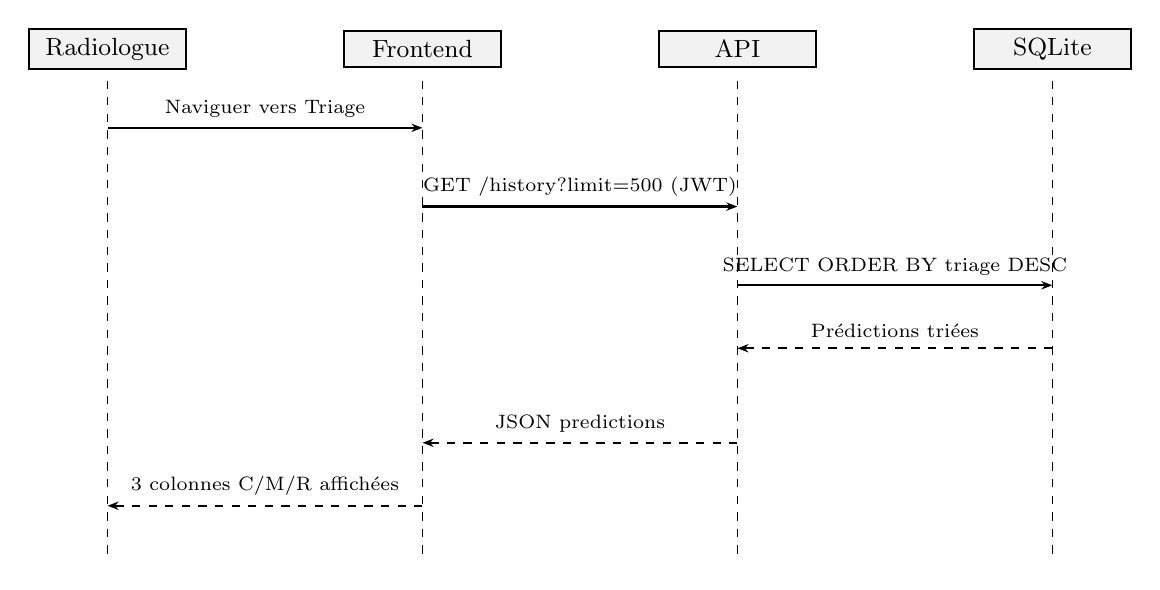
\begin{tikzpicture}[
  every node/.style={font=\small},
  msg/.style={-{Stealth[length=4pt]}, thick},
  ret/.style={-{Stealth[length=4pt]}, thick, dashed},
]
  \node[rectangle,draw,thick,fill=gray!10,minimum width=2cm] (R) at (0,0) {Radiologue};
  \node[rectangle,draw,thick,fill=gray!10,minimum width=2cm] (FE) at (4,0) {Frontend};
  \node[rectangle,draw,thick,fill=gray!10,minimum width=2cm] (BE) at (8,0) {API};
  \node[rectangle,draw,thick,fill=gray!10,minimum width=2cm] (DB) at (12,0) {SQLite};

  \draw[dashed] (0,-0.4) -- (0,-6.5);
  \draw[dashed] (4,-0.4) -- (4,-6.5);
  \draw[dashed] (8,-0.4) -- (8,-6.5);
  \draw[dashed] (12,-0.4) -- (12,-6.5);

  \draw[msg] (0,-1) -- node[above,font=\scriptsize]{Naviguer vers Triage} (4,-1);
  \draw[msg] (4,-2) -- node[above,font=\scriptsize]{GET /history?limit=500 (JWT)} (8,-2);
  \draw[msg] (8,-3) -- node[above,font=\scriptsize]{SELECT ORDER BY triage DESC} (12,-3);
  \draw[ret] (12,-3.8) -- node[above,font=\scriptsize]{Prédictions triées} (8,-3.8);
  \draw[ret] (8,-5) -- node[above,font=\scriptsize]{JSON predictions} (4,-5);
  \draw[ret] (4,-5.8) -- node[above,font=\scriptsize]{3 colonnes C/M/R affichées} (0,-5.8);
\end{tikzpicture}
\caption{Diagramme de séquence --- Consultation du triage}
\end{figure}

\subsection{Consulter le tableau de bord BI}

Dans PneumoScan : \textbf{tableau de bord BI} (admin uniquement).

\begin{figure}[H]
\centering
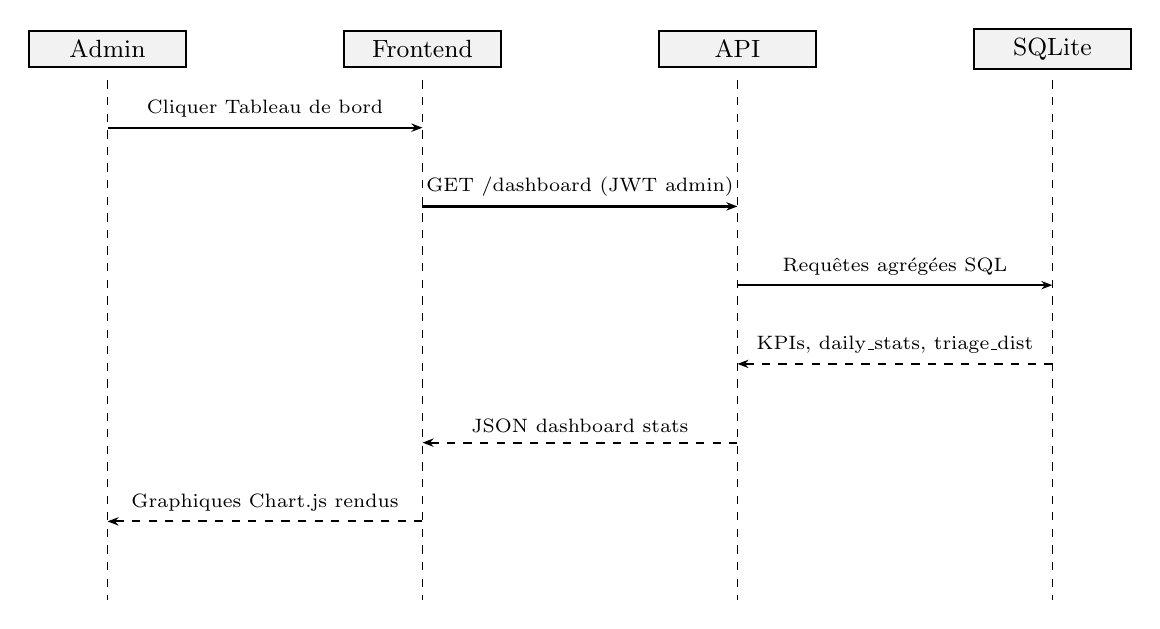
\begin{tikzpicture}[
  every node/.style={font=\small},
  msg/.style={-{Stealth[length=4pt]}, thick},
  ret/.style={-{Stealth[length=4pt]}, thick, dashed},
]
  \node[rectangle,draw,thick,fill=gray!10,minimum width=2cm] (A) at (0,0) {Admin};
  \node[rectangle,draw,thick,fill=gray!10,minimum width=2cm] (FE) at (4,0) {Frontend};
  \node[rectangle,draw,thick,fill=gray!10,minimum width=2cm] (BE) at (8,0) {API};
  \node[rectangle,draw,thick,fill=gray!10,minimum width=2cm] (DB) at (12,0) {SQLite};

  \draw[dashed] (0,-0.4) -- (0,-7);
  \draw[dashed] (4,-0.4) -- (4,-7);
  \draw[dashed] (8,-0.4) -- (8,-7);
  \draw[dashed] (12,-0.4) -- (12,-7);

  \draw[msg] (0,-1) -- node[above,font=\scriptsize]{Cliquer Tableau de bord} (4,-1);
  \draw[msg] (4,-2) -- node[above,font=\scriptsize]{GET /dashboard (JWT admin)} (8,-2);
  \draw[msg] (8,-3) -- node[above,font=\scriptsize]{Requêtes agrégées SQL} (12,-3);
  \draw[ret] (12,-4) -- node[above,font=\scriptsize]{KPIs, daily\_stats, triage\_dist} (8,-4);
  \draw[ret] (8,-5) -- node[above,font=\scriptsize]{JSON dashboard stats} (4,-5);
  \draw[ret] (4,-6) -- node[above,font=\scriptsize]{Graphiques Chart.js rendus} (0,-6);
\end{tikzpicture}
\caption{Diagramme de séquence --- Tableau de bord BI}
\end{figure}

\subsection{Générer un rapport PDF}

Dans PneumoScan : \textbf{anonymisation et génération du rapport PDF}.
Le radiologue active l'anonymisation avant analyse, puis génère le rapport PDF
qui constitue la trace formelle de l'analyse.

\subsection{Diagramme de classe}

\begin{figure}[p]
\centering
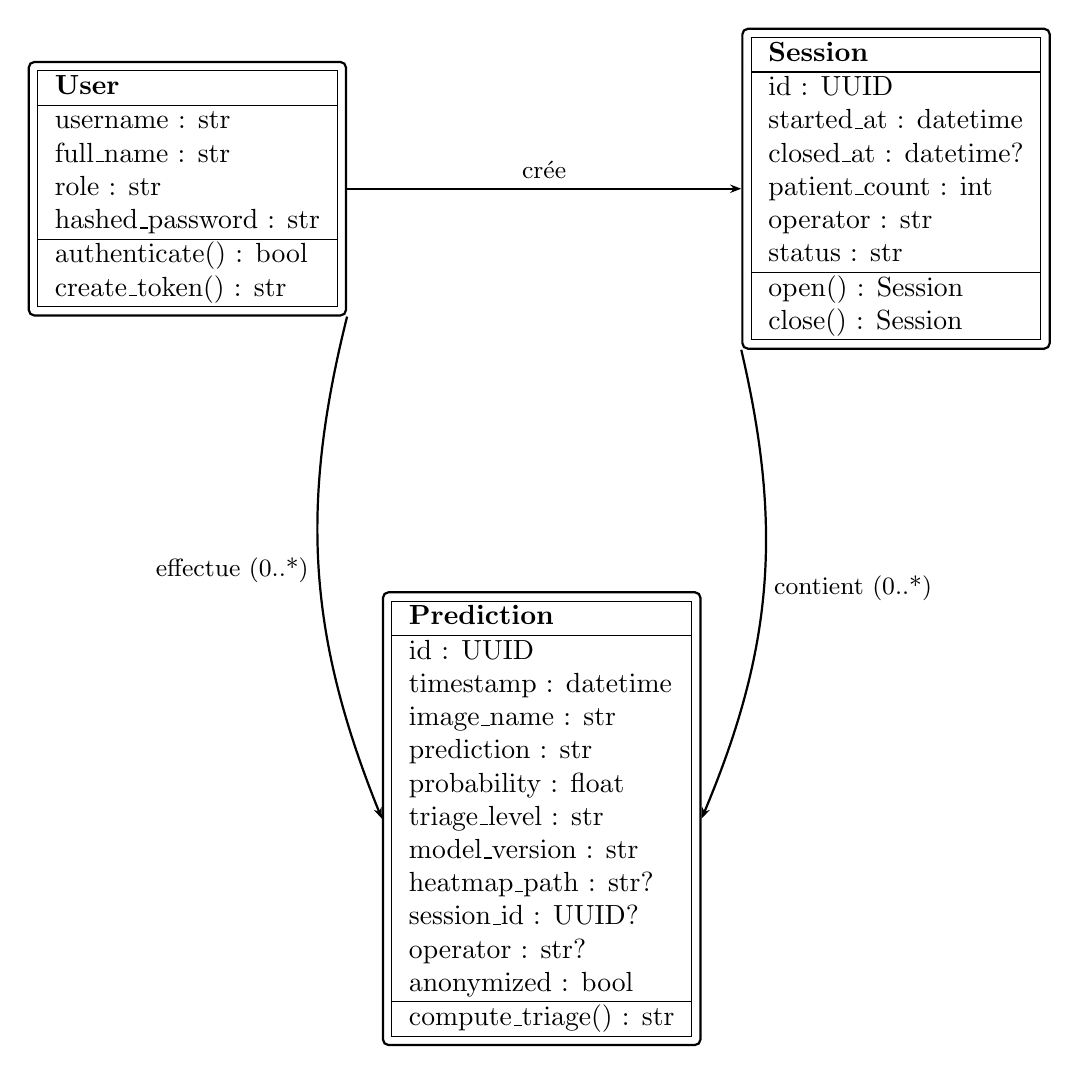
\begin{tikzpicture}[
  every node/.style={font=\normalsize},
  class/.style={rectangle, draw, thick, rounded corners=2pt, fill=white, inner sep=3pt},
  rel/.style={thick, -{Stealth[length=4pt]}},
]
  % Classe User
  \node[class] (user) at (0, 0) {
    \begin{tabular}{|l|}
      \hline
      \textbf{User} \\
      \hline
      username : str \\
      full\_name : str \\
      role : str \\
      hashed\_password : str \\
      \hline
      authenticate() : bool \\
      create\_token() : str \\
      \hline
    \end{tabular}
  };

  % Classe Session
  \node[class] (session) at (9, 0) {
    \begin{tabular}{|l|}
      \hline
      \textbf{Session} \\
      \hline
      id : UUID \\
      started\_at : datetime \\
      closed\_at : datetime? \\
      patient\_count : int \\
      operator : str \\
      status : str \\
      \hline
      open() : Session \\
      close() : Session \\
      \hline
    \end{tabular}
  };

  % Classe Prediction
  \node[class] (pred) at (4.5, -8) {
    \begin{tabular}{|l|}
      \hline
      \textbf{Prediction} \\
      \hline
      id : UUID \\
      timestamp : datetime \\
      image\_name : str \\
      prediction : str \\
      probability : float \\
      triage\_level : str \\
      model\_version : str \\
      heatmap\_path : str? \\
      session\_id : UUID? \\
      operator : str? \\
      anonymized : bool \\
      \hline
      compute\_triage() : str \\
      \hline
    \end{tabular}
  };

  % Relations
  \draw[rel] (user.east) -- node[above, font=\small]{crée} (session.west);
  \draw[rel] (session.south west) to[bend left=18] node[right, font=\small]{contient (0..*)} (pred.east);
  \draw[rel] (user.south east) to[bend right=18] node[left, font=\small]{effectue (0..*)} (pred.west);
\end{tikzpicture}
\caption{Diagramme de classes simplifié}
\end{figure}
\clearpage

\subsection{Dictionnaire des données}

\begin{table}[H]
\centering
\caption{Dictionnaire des données --- Table \texttt{predictions}}
\begin{tabularx}{\textwidth}{L{3cm} L{2.5cm} L{2cm} X}
\toprule
\textbf{Attribut} & \textbf{Type} & \textbf{Contrainte} & \textbf{Description} \\
\midrule
\texttt{id}            & TEXT    & PK, NOT NULL   & Identifiant UUID v4 \\
\texttt{timestamp}     & TEXT    & NOT NULL       & Horodatage ISO 8601 UTC \\
\texttt{image\_name}   & TEXT    & NOT NULL       & Nom du fichier soumis \\
\texttt{prediction}    & TEXT    & NOT NULL       & \texttt{PNEUMONIA} ou \texttt{NORMAL} \\
\texttt{probability}   & REAL    & NOT NULL       & Score de confiance $[0.0, 1.0]$ \\
\texttt{model\_version}& TEXT    & NOT NULL       & Version du modèle utilisé \\
\texttt{heatmap\_path} & TEXT    & NULL OK        & Chemin vers la heatmap HOG \\
\texttt{triage\_level} & TEXT    & NOT NULL       & \texttt{CRITICAL}, \texttt{MODERATE} ou \texttt{ROUTINE} \\
\texttt{session\_id}   & TEXT    & NULL OK, FK    & Référence vers \texttt{sessions.id} \\
\texttt{operator}      & TEXT    & NULL OK        & Nom d'utilisateur de l'opérateur \\
\texttt{anonymized}    & INTEGER & NOT NULL, Def=0& 1 si anonymisée, 0 sinon \\
\bottomrule
\end{tabularx}
\end{table}

\begin{table}[H]
\centering
\caption{Dictionnaire des données --- Table \texttt{sessions}}
\begin{tabularx}{\textwidth}{L{3cm} L{2.5cm} L{2cm} X}
\toprule
\textbf{Attribut} & \textbf{Type} & \textbf{Contrainte} & \textbf{Description} \\
\midrule
\texttt{id}             & TEXT    & PK, NOT NULL      & Identifiant UUID v4 \\
\texttt{started\_at}    & TEXT    & NOT NULL          & Horodatage d'ouverture ISO 8601 \\
\texttt{closed\_at}     & TEXT    & NULL OK           & Horodatage de clôture (NULL si ouverte) \\
\texttt{patient\_count} & INTEGER & NOT NULL          & Nombre de patients prévus \\
\texttt{operator}       & TEXT    & NOT NULL          & Nom d'utilisateur du radiologue \\
\texttt{status}         & TEXT    & NOT NULL, Def=open& \texttt{open} ou \texttt{closed} \\
\bottomrule
\end{tabularx}
\end{table}

\subsection{Le modèle relationnel}

\begin{figure}[H]
\centering
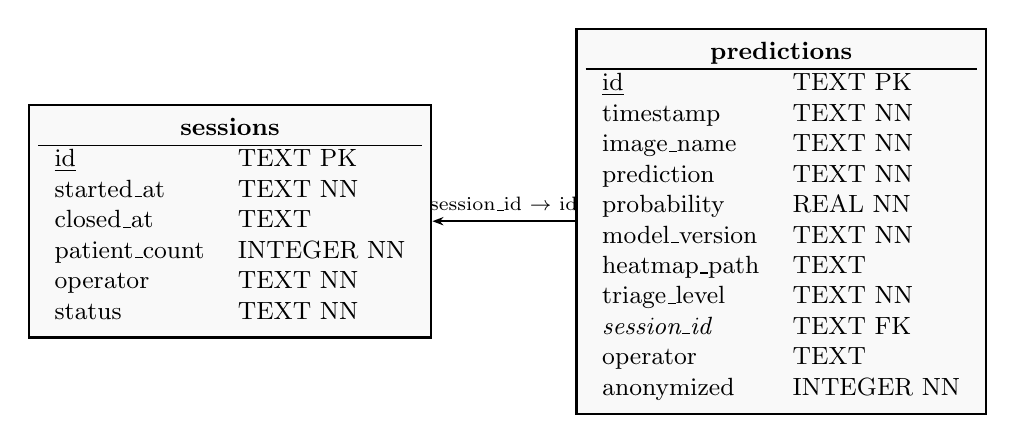
\begin{tikzpicture}[
  every node/.style={font=\small},
  table/.style={rectangle, draw, thick, fill=gray!5},
]
  \node[table] (sessions) at (0,0) {
    \begin{tabular}{ll}
      \multicolumn{2}{c}{\textbf{sessions}} \\
      \hline
      \underline{id}           & TEXT PK \\
      started\_at              & TEXT NN \\
      closed\_at               & TEXT \\
      patient\_count           & INTEGER NN \\
      operator                 & TEXT NN \\
      status                   & TEXT NN \\
    \end{tabular}
  };

  \node[table] (predictions) at (7,0) {
    \begin{tabular}{ll}
      \multicolumn{2}{c}{\textbf{predictions}} \\
      \hline
      \underline{id}           & TEXT PK \\
      timestamp                & TEXT NN \\
      image\_name              & TEXT NN \\
      prediction               & TEXT NN \\
      probability              & REAL NN \\
      model\_version           & TEXT NN \\
      heatmap\_path            & TEXT \\
      triage\_level            & TEXT NN \\
      \textit{session\_id}     & TEXT FK \\
      operator                 & TEXT \\
      anonymized               & INTEGER NN \\
    \end{tabular}
  };

  \draw[thick, -{Stealth[length=4pt]}]
    (predictions.west) -- node[above, font=\scriptsize]{session\_id $\rightarrow$ id}
    (sessions.east);
\end{tikzpicture}
\caption{Modèle relationnel --- Base de données SQLite}
\end{figure}

\subsection{Code SQL}

\begin{lstlisting}[language=SQL, caption={Schéma SQL complet de la base de données}]
-- Table des prédictions
CREATE TABLE IF NOT EXISTS predictions (
    id            TEXT PRIMARY KEY,   -- UUID v4
    timestamp     TEXT NOT NULL,      -- ISO 8601 UTC
    image_name    TEXT NOT NULL,
    prediction    TEXT NOT NULL,      -- 'PNEUMONIA' | 'NORMAL'
    probability   REAL NOT NULL,      -- Confiance [0.0, 1.0]
    model_version TEXT NOT NULL,
    heatmap_path  TEXT,
    triage_level  TEXT NOT NULL,      -- 'CRITICAL' | 'MODERATE' | 'ROUTINE'
    session_id    TEXT,               -- FK -> sessions.id
    operator      TEXT,
    anonymized    INTEGER NOT NULL DEFAULT 0
);

-- Table des sessions de travail
CREATE TABLE IF NOT EXISTS sessions (
    id            TEXT PRIMARY KEY,
    started_at    TEXT NOT NULL,
    closed_at     TEXT,              -- NULL si session ouverte
    patient_count INTEGER NOT NULL,
    operator      TEXT NOT NULL,
    status        TEXT NOT NULL DEFAULT 'open'
);

-- Index pour les filtres fréquents
CREATE INDEX IF NOT EXISTS idx_pred_session
    ON predictions(session_id);
CREATE INDEX IF NOT EXISTS idx_pred_timestamp
    ON predictions(timestamp);
CREATE INDEX IF NOT EXISTS idx_pred_triage
    ON predictions(triage_level);
\end{lstlisting}

\section{Outils, Langages et Environnements de Développement}

\subsection{Langages de Programmation}

\begin{table}[H]
\centering
\caption{Langages de programmation utilisés}
\begin{tabularx}{\textwidth}{L{3cm} L{3cm} X}
\toprule
\textbf{Langage} & \textbf{Version} & \textbf{Usage dans le projet} \\
\midrule
Python  & 3.11 & Backend API, pipeline ML, tests unitaires \\
JavaScript & ES2022 & Frontend Vue.js 3, génération PDF \\
SQL     & SQLite 3 & Requêtes BDD, agrégations BI \\
\bottomrule
\end{tabularx}
\end{table}

\subsection{Frameworks et Bibliothèques}

\begin{table}[H]
\centering
\caption{Frameworks et bibliothèques}
\begin{tabularx}{\textwidth}{L{3cm} L{2.5cm} X}
\toprule
\textbf{Outil} & \textbf{Version} & \textbf{Rôle} \\
\midrule
FastAPI   & 0.111 & Framework API REST asynchrone \\
Vue.js    & 3.x (CDN) & Framework frontend réactif \\
scikit-learn + PyTorch & 1.5.0 / 2.x & Pipeline EfficientNet-B0 + SVM (\binpart) \\
OpenCV    & 4.9.0 & Prétraitement images, garde OOD, heatmap \\
scikit-image & 0.22.0 & Extraction du descripteur HOG \\
Pillow    & 10.3.0 & Ouverture et conversion des images \\
Chart.js  & 4.4.0 & Graphiques tableau de bord BI \\
jsPDF     & 2.5.1 & Génération de rapports PDF côté client \\
pytest    & 8.2.0 & Tests unitaires (31 cas, 5 classes) \\
python-jose & 3.3.0 & Encodage/décodage JWT HS256 \\
passlib   & 1.7.4 & Hachage bcrypt des mots de passe \\
\bottomrule
\end{tabularx}
\end{table}

\subsection{Base de Données}

SQLite 3 a été retenu pour le prototype : léger, sans serveur dédié,
embarqué dans Python via le module standard \texttt{sqlite3}.
Le schéma comporte 2 tables et 3 index. La connexion est gérée
par un gestionnaire de contexte Python (\texttt{@contextmanager})
garantissant la fermeture et le rollback en cas d'exception.

\subsection{Communication en Temps Réel}

La communication entre le frontend et le backend est réalisée par des appels
\textbf{HTTP/REST} standard (fetch API). La mise à jour de la file de triage
est déclenchée explicitement par le radiologue (bouton ``Actualiser''),
sans connexion persistante WebSocket dans cette version prototype.

\subsection{Déploiement et Hébergement}

\begin{infobox}[Point central de la démonstration]
Le déploiement conteneurisé via \texttt{Docker Compose} constitue un axe majeur
de la soutenance : il démontre la reproductibilité, la portabilité et la capacité
d'industrialisation du prototype au-delà de la simple preuve de concept algorithmique.
\end{infobox}

\begin{table}[H]
\centering
\caption{Configuration Docker Compose}
\begin{tabularx}{\textwidth}{L{3.5cm} L{2cm} X}
\toprule
\textbf{Service} & \textbf{Port} & \textbf{Description} \\
\midrule
\texttt{pneumoscan-backend}  & 8000 & API FastAPI --- Python 3.11-slim + dépendances ML \\
\texttt{pneumoscan-frontend} & 3000 & Interface Vue.js servie par Nginx Alpine (hôte) \\
\bottomrule
\end{tabularx}
\end{table}

\begin{lstlisting}[language=bash, caption={Déploiement en trois commandes}]
# 1. Placer le modèle entraîné (contribution du binôme)
cp pneumonia_hog_model.pkl ./backend/model/

# 2. Construire et démarrer les deux services
docker compose up --build

# 3. Accéder à l'application
# Interface : http://localhost:3000
# Documentation API : http://localhost:8000/docs
\end{lstlisting}

\subsection{Stockage des fichiers}

Les heatmaps HOG générées sont stockées sur le disque dans le répertoire
\texttt{/app/heatmaps/} (volume Docker persistant). Chaque fichier est nommé
\texttt{heatmap\_\{uuid\_hex\}.png} et servi statiquement via l'endpoint
\texttt{GET /heatmap/\{filename\}}.

\subsection{Environnements de Développement}

\begin{table}[H]
\centering
\caption{Environnement de développement}
\begin{tabularx}{\textwidth}{L{3.5cm} X}
\toprule
\textbf{Outil} & \textbf{Usage} \\
\midrule
VS Code           & Éditeur principal (extensions Python, Pylance, Docker) \\
Git / GitHub      & Versioning, collaboration, \href{https://github.com/Anis-Aissani}{\texttt{github.com/Anis-Aissani}} \\
Docker Desktop    & Exécution et test des conteneurs en local \\
Postman           & Test et débogage des endpoints API \\
Jupyter Notebook  & Exploration du dataset et entraînement du modèle (\binpart) \\
\bottomrule
\end{tabularx}
\end{table}

\section{Description des Résultats Attendus}

\begin{table}[H]
\centering
\caption{Résultats attendus du système}
\begin{tabularx}{\textwidth}{L{4cm} X}
\toprule
\textbf{Fonctionnalité} & \textbf{Résultat attendu} \\
\midrule
Analyse d'une radiographie & Label (PNEUMONIA / NORMAL), score de confiance, niveau de triage, heatmap HOG \\
Triage automatique & File de travail triée Critical $\rightarrow$ Moderate $\rightarrow$ Routine \\
Rejet OOD & HTTP 400 avec message d'erreur explicite pour toute image non radiographique \\
Authentification & Token JWT valide retourné en $<$ 500ms \\
Rapport PDF & Document A4 structuré, grille rigide, images côte-à-côte \\
Tableau de bord BI & KPIs mis à jour en temps réel, graphiques Chart.js \\
Tests unitaires & 32 tests passants en $<$ 30 secondes \\
Déploiement & Application accessible sur http://localhost:3000 après \texttt{docker compose up} \\
\bottomrule
\end{tabularx}
\end{table}

% ============================================================
% CONCLUSION GENERALE
% ============================================================
\chapter*{Conclusion générale}
\addcontentsline{toc}{chapter}{Conclusion générale}

PneumoScan réalise l'objectif qui lui était assigné : concevoir et développer
une architecture logicielle complète intégrant un composant d'intelligence
artificielle pré-entraîné dans un contexte médical réaliste.

Le cadre \acrshort{up} a structuré l'avancement selon la séquence suivante :
Inception (2 sem.), Élaboration (4 sem.), Construction (8 sem.), Transition (2 sem.).
Cette progression a permis de synchroniser la contribution modèle du binôme et
ma contribution applicative jusqu'au déploiement final.

\vspace{8pt}
\noindent Les contributions personnelles du projet (ma partie) comprennent :
\begin{enumerate}
  \item Un \textbf{pipeline applicatif robuste} avec garde OOD OpenCV,
        résolvant le problème des faux positifs sur images non radiographiques.
  \item Une \textbf{architecture sécurisée} (JWT HS256, RBAC, sessions anti-zombie)
        respectant les bonnes pratiques de sécurité des applications web.
  \item Une \textbf{interface utilisateur} Vue.js 3 responsive, avec file de triage,
        contrôles d'image, génération de PDF et tableau de bord BI.
  \item Une \textbf{suite de tests automatisés} (32 cas pytest) couvrant les
        composants critiques.
  \item Un \textbf{déploiement conteneurisé} reproductible via Docker Compose.
\end{enumerate}

\vspace{6pt}
\noindent Les perspectives d'évolution prioritaires identifiées sont :
\begin{itemize}
  \item Intégration du support \textbf{DICOM} pour les fichiers hospitaliers réels
  \item Fine-tuning du pipeline \textbf{EfficientNet-B0 + SVM} sur données plus diversifiées
  \item Implémentation de méthodes d'explicabilité (\textbf{Grad-CAM}, SHAP)
  \item Migration vers \textbf{PostgreSQL} pour un déploiement multi-utilisateurs
\end{itemize}

\vspace{6pt}
Ce projet m'a permis de mettre en œuvre l'ensemble du cycle de développement
logiciel --- de la conception UML au déploiement Docker ---
en intégrant le modèle produit par mon binôme dans l'application que j'ai
construite, tout en confrontant les défis réels de l'intégration d'un composant IA
dans une architecture applicative professionnelle.

% ============================================================
% RESUME ET MOTS-CLES
% ============================================================
\chapter*{Résumé}
\addcontentsline{toc}{chapter}{Résumé}

\textbf{Résumé :}
PneumoScan est un système web d'aide au triage des radiographies thoraciques,
développé dans le cadre d'un projet annuel de Licence Informatique (L3)
à l'Université de Rouen Normandie. Le système intègre un pipeline de machine
learning (EfficientNet-B0 + SVM, Accuracy 86.2\% / F1 88.4\%) dans une architecture logicielle
complète : API REST FastAPI, interface Vue.js 3, base de données SQLite,
authentification JWT/RBAC et déploiement Docker Compose. Une garde
hors-distribution (OOD) basée sur OpenCV rejette les images non radiographiques
avant toute inférence. L'interface propose une file de triage automatique
(Critical / Moderate / Routine), un tableau de bord BI et la génération
de rapports PDF structurés.

\vspace{8pt}
\noindent\textbf{Mots-clés :} Intelligence Artificielle, Machine Learning,
HOG, SVM, Triage Médical, FastAPI, Vue.js, JWT, Docker, SQLite,
Radiographie Thoracique, Pneumonie, Out-Of-Distribution.

% ============================================================
% LISTE DES MOTS-CLES ET DEFINITIONS
% ============================================================
\chapter*{Liste des mots-clés et leurs définitions}
\addcontentsline{toc}{chapter}{Liste des mots-clés et leurs définitions}

\begin{description}
  \item[\acrshort{hog} (Histogram of Oriented Gradients)]
    Descripteur de features locales calculant la distribution des orientations
    des gradients dans des cellules d'une image \cite{dalal2005}.
  \item[\acrshort{svm} (Support Vector Machine)]
    Classifieur supervisé cherchant l'hyperplan de marge maximale
    entre deux classes \cite{cortes1995}.
  \item[\acrshort{jwt} (JSON Web Token)]
    Standard RFC 7519 pour transmettre des informations signées entre parties
    sous forme de token compact \cite{jones2015}.
  \item[\acrshort{rbac} (Role-Based Access Control)]
    Modèle de contrôle d'accès attribuant des permissions à des rôles,
    eux-mêmes attribués à des utilisateurs \cite{sandhu1996}.
  \item[\acrshort{ood} (Out-Of-Distribution)]
    Données ne ressemblant pas à celles vues à l'entraînement,
    pouvant provoquer des prédictions erronées à haute confiance.
  \item[\acrshort{pacs} (Picture Archiving and Communication System)]
    Système hospitalier de stockage et distribution des images médicales.
  \item[API REST]
    Interface de programmation basée sur les principes REST (Representational
    State Transfer) définis par Fielding \cite{fielding2000}.
  \item[Docker Compose]
    Outil d'orchestration de conteneurs Docker permettant de définir
    et démarrer des applications multi-services.
  \item[Triage clinique]
    Processus médical de classification des patients selon l'urgence
    de leur prise en charge.
\end{description}

% ============================================================
% BIBLIOGRAPHIE
% ============================================================
\begin{thebibliography}{99}
\addcontentsline{toc}{chapter}{Bibliographie}

\bibitem{cortes1995}
C.~Cortes, V.~Vapnik.
\textit{Support-vector networks}.
Machine Learning, 20(3), pp.~273--297, 1995.

\bibitem{dalal2005}
N.~Dalal, B.~Triggs.
\textit{Histograms of Oriented Gradients for Human Detection}.
IEEE Conference on Computer Vision and Pattern Recognition (CVPR),
pp.~886--893, 2005.

\bibitem{fielding2000}
R.~T.~Fielding.
\textit{Architectural Styles and the Design of Network-based Software Architectures}.
Thèse de doctorat, Université de Californie, Irvine, 2000.

\bibitem{goodfellow2016}
I.~Goodfellow, Y.~Bengio, A.~Courville.
\textit{Deep Learning}.
MIT Press, 2016.

\bibitem{huang2017}
G.~Huang, Z.~Liu, L.~van~der~Maaten, K.~Q.~Weinberger.
\textit{Densely Connected Convolutional Networks}.
IEEE CVPR, pp.~4700--4708, 2017.

\bibitem{jones2015}
M.~Jones, J.~Bradley, N.~Sakimura.
\textit{JSON Web Token (JWT)}.
RFC~7519, IETF, 2015.

\bibitem{mooney2018}
P.~Mooney.
\textit{Chest X-Ray Images (Pneumonia)}.
Kaggle, 2018.
\url{https://www.kaggle.com/datasets/paultimothymooney/chest-xray-pneumonia}

\bibitem{mdr2017}
Parlement européen et Conseil de l'UE.
\textit{Règlement (UE) 2017/745 relatif aux dispositifs médicaux (MDR)}.
Journal officiel de l'Union européenne, L~117, 2017.

\bibitem{provos1999}
N.~Provos, D.~Mazieres.
\textit{A Future-Adaptable Password Scheme}.
USENIX Annual Technical Conference, 1999.

\bibitem{rajpurkar2017}
P.~Rajpurkar et al.
\textit{CheXNet: Radiologist-Level Pneumonia Detection on Chest X-Rays
with Deep Learning}.
arXiv:1711.05225, 2017.

\bibitem{rgpd2016}
Parlement européen et Conseil de l'UE.
\textit{Règlement (UE) 2016/679 --- Protection des données à caractère personnel (RGPD)}.
Journal officiel de l'Union européenne, L~119, 2016.

\bibitem{samek2019}
W.~Samek, K.-R.~Müller.
\textit{Explainable Artificial Intelligence: Understanding, Visualizing
and Interpreting Deep Neural Network Predictions}.
ITU Journal, vol.~1, 2019.

\bibitem{sandhu1996}
R.~S.~Sandhu, E.~J.~Coyne, H.~L.~Feinstein, C.~E.~Youman.
\textit{Role-Based Access Control Models}.
IEEE Computer, 29(2), pp.~38--47, 1996.

\bibitem{scikit2011}
F.~Pedregosa et al.
\textit{Scikit-learn: Machine Learning in Python}.
Journal of Machine Learning Research, 12, pp.~2825--2830, 2011.

\bibitem{selvaraju2017}
R.~R.~Selvaraju, M.~Cogswell, A.~Das, R.~Vedantam, D.~Parikh, D.~Batra.
\textit{Grad-CAM: Visual Explanations from Deep Networks
via Gradient-based Localization}.
IEEE ICCV, pp.~618--626, 2017.

\bibitem{who2022}
Organisation mondiale de la Santé (OMS).
\textit{Pneumonia --- Key Facts}.
World Health Organization, 2022.
\url{https://www.who.int/news-room/fact-sheets/detail/pneumonia}

\bibitem{binome2026model}
M.~Elakef Zenagui.
\textit{Artefact modèle de classification pneumonie utilisé pour l'intégration API de PneumoScan}.
Google Drive, 2026.
\url{https://drive.google.com/file/d/1CH2zGzIfj5EJY3V_-bXOqAYCs7CbaPfN/view?usp=sharing}

\end{thebibliography}

\printglossaries
\ifquickbuild\else
\printglossaries
\fi

\end{document}